\section{Additional figures}\label{app:figs}

This appendix expands \cref{fig:qual_main,fig:spectrum_main} and holds the development figures behind \cref{sec:checkpoint,sec:papercode}. \Cref{fig:qual} shows held-out samples, \cref{fig:checkpoint} the development checkpoint diagnostic, \cref{fig:spectrum} the octave-band spectra, and \cref{fig:papercode} the development paper-versus-code comparison.

\begin{figure}[H]
\centering
\figorplaceholder[\linewidth]{figs/f4_qualitative.pdf}{3.1in}
\caption{\textbf{\ntk{} loses fine detail at $4096^2$.} The other arms render comparable detail, and \dype{} shows faint speckle in flat sky on held-out row 8 (one crop checked); compositions differ between arms, so a crop can show different content. Held-out rows 8, 9 and 10 (left to right), the first three held-out rows, were fixed before any output was viewed; seed 0, one sample per arm. Full frames are Lanczos-reduced; native-resolution crops sit at identical coordinates and are never resampled (red: highest-detail tile of the across-arm mean luminance; cyan: image center). Prompts, left to right: ``A stone bridge with arched spans reflects golden light on the water, flanked by buildings and a leafy tree under a clear blue sky.'' ``A panoramic view of Paris featuring the Eiffel Tower, the Seine River, and various ornate buildings with greenery and bustling activity, including boats on the water and crowds along walkways.'' ``A cluttered artist's corner features an ornate gold frame, a painting of a man with glasses, several empty picture frames, a vintage suitcase, and various brushes in a tin can, all set against a textured gray wall and draped with patterned fabric.''}
\label{fig:qual}
\end{figure}

\begin{figure}[H]
\centering
\figorplaceholder[\linewidth]{figs/f5_checkpoint.pdf}{3.26in}
\caption{\textbf{Lattice and checkpoint check.} The development comparison shows a lattice on \fluxdev{}, but checkpoint and guidance both change. (a)~Dev prompt 0 under official \dype{} code (seed 42) and our \dype{} and \segaofficial{} pipelines (seed 0), at guidance 3.5 (\fluxdev) and 4.5 (\krea). Red and cyan boxes mark native 192-pixel windows at the same place in every image. (b)~Whitened radial power spectra of luminance: \fluxdev{} (black) peaks at the lattice period (dot) and \krea{} (gray) does not in these samples. Peak ratios: 36$\times$ for the official-code pair; over eight prompts in our pipeline, 12$\times$ [7, 20] for \dype{} and 5$\times$ [2, 11] for \segaofficial{} (geometric means, 95\% bootstrap intervals). Official-code evidence covers one prompt per checkpoint, and the figure does not isolate a checkpoint effect.}
\label{fig:checkpoint}
\end{figure}

\begin{figure}[H]
\centering
\figorplaceholder[\linewidth]{figs/f8_spectrum.pdf}{2.2in}
\caption{\textbf{Spectra against references and \sega.} Without \sega's per-band allocation, luminance power at 8 to 32 pixel wavelengths (gray band) sits above released \sega's; \constancytm{} leaves a similar excess, and \ntk{} falls short from 8 to 1024 pixels. (a)~Log-power error against the mean $\ln P$ of the 195 \afk{} references, per octave band of linear-sRGB luminance; (b)~paired difference from \segaofficial, the dashed blue zero line; positive means more power. Held-out rows 8--194 ($n=\N{ho@nprompts}$, seed 0) with 95\% bootstrap intervals over prompts; the dashed vertical marks the Nyquist frequency of a 224-pixel view.}
\label{fig:spectrum}
\end{figure}

\begin{figure}[H]
\centering
\figorplaceholder[\linewidth]{figs/f6_sega_code.pdf}{2.4in}
\caption{\textbf{Printed equations against the release.} The printed-law implementation produces larger gain changes than the release and degrades this development pilot. Eight dev prompts (rows 0--7, seed 0), descriptive only. (a)~Median log logit gain per rotary pair (pair 0 has the highest frequency) and denoising step. Released and printed-law heatmaps have separate symmetric color scales, so equal colors across the groups do not mean equal magnitudes. The line panel uses one shared axis for mean log gain over prompts, steps and both spatial axes; static variants (dashed) average each method's gains over prompts and steps. (b)~Dev prompt 0, seed 0: full frames and a native-resolution crop (red box). \Cref{tab:papercode_scores} gives CLIP score and ImageReward means over the eight dev prompts, with paired differences from \segaofficial{} and 95\% bootstrap intervals.}
\label{fig:papercode}
\end{figure}

\clearpage

\section{Full held-out results}\label{app:full}

This appendix expands \cref{tab:results}: \cref{tab:main} gives its paired differences with intervals, \cref{tab:share} the decomposition with means, \cref{tab:means_full,tab:deltas_full} all ten metrics and \cref{tab:octave} the spectral bands.

\begin{table}[!htbp]
\centering
\caption{\textbf{Paired held-out differences (expands \cref{tab:results}).} Held-out paired differences against \segaofficial{} (rows 8--194, seed 0, $n=\N{ho@nprompts}$); the first row gives the absolute means of \segaofficial. Each cell shows the mean difference and its nominal 95\% bootstrap interval; \better{}/\worse{} mark intervals that exclude zero in the better or worse direction; unmarked cells are ties. A star marks a Holm-adjusted $p\le0.05$ across this table's paired comparisons, using approximate centered-bootstrap tests. \Cref{tab:deltas_full} has all ten metrics and a separate Holm family. Key result: base and temperature carry most of \sega's gain, and no per-band law beats it.}
\label{tab:main}
\footnotesize
\setlength{\tabcolsep}{3.1pt}
\begin{tabular}{@{}l rrrrrr@{}}
\toprule
Method & \makecell[r]{Image-\\Reward$\uparrow$} & \makecell[r]{Pick-\\Score$\uparrow$} & \makecell[r]{CLIP\\score$\uparrow$} & \makecell[r]{MUSIQ\\full$\uparrow$} & \makecell[r]{MUSIQ\\crop$\uparrow$} & \makecell[r]{CLIP-IQA\\full$\uparrow$} \\
\midrule
\segaofficial{} & \refcell{1.190} & \refcell{23.05} & \refcell{29.14} & \refcell{45.23} & \refcell{58.33} & \refcell{0.603} \\
\midrule
\multicolumn{7}{@{}l}{\emph{Decomposition of \segaofficial}} \\[1pt]
\ntk{} & \dcellW{-0.594}{-0.701}{-0.494} & \dcellW{-1.02}{-1.16}{-0.89} & \dcellW{-1.99}{-2.43}{-1.55} & \dcellW{-15.74}{-17.50}{-14.00} & \dcellW{-18.70}{-20.68}{-16.86} & \dcellW{-0.046}{-0.062}{-0.031} \\
\tempsb{} & \dcellT{+0.026}{-0.016}{+0.070} & \dcellT{+0.03}{-0.03}{+0.09} & \dcellT{+0.02}{-0.19}{+0.23} & \dcellW{-2.09}{-3.25}{-0.96} & \dcellT{-0.11}{-0.71}{+0.51} & \dcellW{-0.009}{-0.018}{-0.001} \\
\addlinespace[2pt]
\multicolumn{7}{@{}l}{\emph{Other baseline}} \\[1pt]
\dype{} & \dcellW{-0.164}{-0.258}{-0.087} & \dcellW{-0.49}{-0.63}{-0.36} & \dcellW{-0.37}{-0.72}{-0.01} & \dcellW{-1.88}{-3.26}{-0.56} & \dcellB{+1.97}{+1.16}{+2.80} & \dcellB{+0.029}{+0.020}{+0.038} \\
\addlinespace[2pt]
\multicolumn{7}{@{}l}{\emph{Principled per-band laws (ours)}} \\[1pt]
\constancytm{} & \dcellT{+0.018}{-0.023}{+0.059} & \dcellT{-0.05}{-0.11}{+0.02} & \dcellW{-0.27}{-0.49}{-0.04} & \dcellW{-3.04}{-4.28}{-1.81} & \dcellW{-2.19}{-2.81}{-1.57} & \dcellW{-0.025}{-0.034}{-0.017} \\
\segactm{} & \dcellT{+0.009}{-0.008}{+0.027} & \dcellW{-0.08}{-0.10}{-0.05} & \dcellW{-0.09}{-0.20}{+0.00} & \dcellT{-0.21}{-0.71}{+0.32} & \dcellW{-1.13}{-1.39}{-0.90} & \dcellT{+0.003}{+0.000}{+0.006} \\
\bottomrule
\end{tabular}

\end{table}

\Cref{tab:share} decomposes \sega's gain over \ntk{} with means and paired gains, \cref{tab:means_full} gives absolute means and \cref{tab:deltas_full} the paired differences for all ten metrics. The spectral rows use the mean octave profile of the 195 \afk{} reference images as the target; \cref{tab:octave} breaks the spectral error into its 11 octave bands. FID and KID are not tabulated: for the seed-1 images (\N{fid@n} prompts per arm, including one dev row), the paired FID difference of \tempsb{} against \segaofficial{} is \N{fid@tsb@fid} with interval \N{fid@tsb@fid@ci}, and that of \constancytm{} is \N{fid@ctm@fid} with interval \N{fid@ctm@fid@ci}.

In band 7, \ntk{} falls below the reference profile (log-power error \N{oct@ntk@b7}); the two arms with \sega's allocation stay closest to it (\segaofficial{} \N{oct@sega@b7}, \segactm{} \N{oct@sctm@b7}), and \tempsb{} carries excess power (\N{oct@tsb@b7}). These held-out spectral differences lie above the Nyquist limit of the 224-pixel reward-model view (\cref{sec:pitfalls}).

\begin{table}[!htbp]
\centering
\caption{\textbf{Where \sega's improvement over \ntk{} comes from.} Means on the same \N{sh@n} held-out prompts, paired gains from base and temperature and from the allocation, and the share of the total gain carried by base and temperature, (\tempsb{} $-$ \ntk)/(\segaofficial{} $-$ \ntk), with its 95\% paired bootstrap interval. A share above 100\% means the allocation's point estimate is negative.}
\label{tab:share}
\footnotesize
\setlength{\tabcolsep}{4pt}
\begin{tabular}{@{}l rrr rr r@{}}
\toprule
 & \multicolumn{3}{c}{Mean ($n=187$)} & \multicolumn{2}{c}{Paired gain} & \\
\cmidrule(lr){2-4}\cmidrule(lr){5-6}
Metric & \ntkH & \tempsbH & \segaofficialH & \hdr{base\\+\,temp.} & \hdr{alloc-\\ation} & \hdr{share of\\base\,+\,temp.} \\
\midrule
ImageReward$\uparrow$ & $0.596$ & $1.216$ & $1.190$ & \dcellB{+0.620}{+0.525}{+0.724} & \dcellT{-0.026}{-0.070}{+0.016} & 104\% {\fontsize{6.5}{7}\selectfont[97, 113]} \\
PickScore$\uparrow$ & $22.03$ & $23.08$ & $23.05$ & \dcellB{+1.05}{+0.92}{+1.18} & \dcellT{-0.03}{-0.09}{+0.03} & 103\% {\fontsize{6.5}{7}\selectfont[97, 109]} \\
CLIP$\uparrow$ & $27.15$ & $29.15$ & $29.14$ & \dcellB{+2.01}{+1.57}{+2.48} & \dcellT{-0.02}{-0.23}{+0.19} & 101\% {\fontsize{6.5}{7}\selectfont[90, 112]} \\
MUSIQ$\uparrow$ & $29.49$ & $43.14$ & $45.23$ & \dcellB{+13.65}{+12.05}{+15.28} & \dcellB{+2.09}{+0.96}{+3.25} & 87\% {\fontsize{6.5}{7}\selectfont[80, 94]} \\
MUSIQ\textsubscript{crop}$\uparrow$ & $39.63$ & $58.22$ & $58.33$ & \dcellB{+18.59}{+16.72}{+20.63} & \dcellT{+0.11}{-0.51}{+0.71} & 99\% {\fontsize{6.5}{7}\selectfont[96, 103]} \\
CLIP-IQA$\uparrow$ & $0.557$ & $0.594$ & $0.603$ & \dcellB{+0.037}{+0.021}{+0.053} & \dcellB{+0.009}{+0.001}{+0.018} & 80\% {\fontsize{6.5}{7}\selectfont[59, 98]} \\
\bottomrule
\end{tabular}

\end{table}

\begin{table}[!htbp]
\centering
\caption{\textbf{Held-out means with 95\% bootstrap intervals} (rows 8--194, seed 0). \constancy{} is the partial run on \hon{cons} prompts (\cref{app:partial}).}
\label{tab:means_full}
\scriptsize
\setlength{\tabcolsep}{1.3pt}
\begin{tabular}{@{}lrrrrrrr@{}}
\toprule
Metric & \segaofficialH & \ntkH & \tempsbH & \dypeH & \constancyH & \constancytmH & \segactmH \\
 & \tiny $n=187$ & \tiny $n=187$ & \tiny $n=187$ & \tiny $n=187$ & \tiny $n=41$ & \tiny $n=187$ & \tiny $n=187$ \\
\midrule
ImageReward$\uparrow$ & \mcell{1.190}{1.087}{1.284} & \mcell{0.596}{0.456}{0.736} & \mcell{1.216}{1.118}{1.313} & \mcell{1.026}{0.910}{1.142} & \mcell{1.177}{0.953}{1.392} & \mcell{1.208}{1.110}{1.304} & \mcell{1.199}{1.096}{1.293} \\
PickScore$\uparrow$ & \mcell{23.05}{22.89}{23.21} & \mcell{22.03}{21.84}{22.21} & \mcell{23.08}{22.92}{23.24} & \mcell{22.57}{22.36}{22.75} & \mcell{22.70}{22.29}{23.08} & \mcell{23.01}{22.84}{23.16} & \mcell{22.98}{22.81}{23.13} \\
CLIP$\uparrow$ & \mcell{29.14}{28.70}{29.55} & \mcell{27.15}{26.64}{27.64} & \mcell{29.15}{28.72}{29.58} & \mcell{28.76}{28.32}{29.20} & \mcell{29.46}{28.40}{30.49} & \mcell{28.87}{28.42}{29.31} & \mcell{29.04}{28.61}{29.47} \\
MUSIQ$\uparrow$ & \mcell{45.23}{43.69}{46.79} & \mcell{29.49}{28.13}{30.95} & \mcell{43.14}{41.58}{44.61} & \mcell{43.35}{41.71}{45.02} & \mcell{40.55}{37.20}{43.56} & \mcell{42.19}{40.65}{43.58} & \mcell{45.02}{43.56}{46.53} \\
MUSIQ\textsubscript{crop}$\uparrow$ & \mcell{58.33}{57.06}{59.63} & \mcell{39.63}{37.77}{41.33} & \mcell{58.22}{57.07}{59.44} & \mcell{60.30}{59.12}{61.53} & \mcell{60.75}{58.19}{63.01} & \mcell{56.14}{54.98}{57.36} & \mcell{57.20}{55.84}{58.52} \\
CLIP-IQA$\uparrow$ & \mcell{0.603}{0.590}{0.616} & \mcell{0.557}{0.546}{0.568} & \mcell{0.594}{0.581}{0.607} & \mcell{0.632}{0.618}{0.645} & \mcell{0.572}{0.544}{0.601} & \mcell{0.578}{0.566}{0.590} & \mcell{0.606}{0.593}{0.619} \\
CLIP-IQA\textsubscript{crop}$\uparrow$ & \mcell{0.586}{0.573}{0.600} & \mcell{0.537}{0.525}{0.549} & \mcell{0.569}{0.556}{0.583} & \mcell{0.599}{0.585}{0.613} & \mcell{0.543}{0.514}{0.572} & \mcell{0.550}{0.538}{0.563} & \mcell{0.588}{0.576}{0.602} \\
Spec.\ err.$\downarrow$ & \mcell{1.068}{1.005}{1.133} & \mcell{1.285}{1.214}{1.358} & \mcell{1.102}{1.035}{1.168} & \mcell{1.096}{1.024}{1.168} & \mcell{1.337}{1.205}{1.477} & \mcell{1.088}{1.020}{1.152} & \mcell{1.066}{1.001}{1.133} \\
Slope err.$\downarrow$ & \mcell{0.200}{0.180}{0.221} & \mcell{0.165}{0.146}{0.185} & \mcell{0.224}{0.200}{0.247} & \mcell{0.218}{0.194}{0.242} & \mcell{0.276}{0.218}{0.338} & \mcell{0.218}{0.195}{0.240} & \mcell{0.197}{0.178}{0.218} \\
Tiling$\downarrow$ & \mcell{0.0684}{0.0568}{0.0802} & \mcell{0.0757}{0.0612}{0.0905} & \mcell{0.0616}{0.0507}{0.0732} & \mcell{0.0865}{0.0778}{0.0953} & \mcell{0.0589}{0.0390}{0.0797} & \mcell{0.0616}{0.0505}{0.0732} & \mcell{0.0684}{0.0566}{0.0804} \\
\bottomrule
\end{tabular}

\end{table}

\begin{table}[!htbp]
\centering
\caption{\textbf{Held-out paired differences against \segaofficial{}, all metrics.} Nominal 95\% intervals and direction triangles as in \cref{tab:main}; stars mark approximate Holm-adjusted $p\le0.05$ across all paired comparisons in this table. \constancy{} is the partial run on \hon{cons} prompts (\cref{app:partial}).}
\label{tab:deltas_full}
\scriptsize
\setlength{\tabcolsep}{1.8pt}
\begin{tabular}{@{}lrrrrrr@{}}
\toprule
Metric & \ntkH & \tempsbH & \dypeH & \constancyH & \constancytmH & \segactmH \\
 & \tiny $n=187$ & \tiny $n=187$ & \tiny $n=187$ & \tiny $n=41$ & \tiny $n=187$ & \tiny $n=187$ \\
\midrule
ImageReward$\uparrow$ & \dcellW{-0.594}{-0.701}{-0.494} & \dcellT{+0.026}{-0.016}{+0.070} & \dcellW{-0.164}{-0.258}{-0.087} & \dcellT{+0.018}{-0.089}{+0.133} & \dcellT{+0.018}{-0.023}{+0.059} & \dcellT{+0.009}{-0.008}{+0.027} \\
PickScore$\uparrow$ & \dcellW{-1.02}{-1.16}{-0.89} & \dcellT{+0.03}{-0.03}{+0.09} & \dcellW{-0.49}{-0.63}{-0.36} & \dcellT{-0.07}{-0.28}{+0.18} & \dcellT{-0.05}{-0.11}{+0.02} & \dcellW{-0.08}{-0.10}{-0.05} \\
CLIP$\uparrow$ & \dcellW{-1.99}{-2.43}{-1.55} & \dcellT{+0.02}{-0.19}{+0.23} & \dcellW{-0.37}{-0.72}{-0.01} & \dcellT{-0.05}{-0.78}{+0.68} & \dcellW{-0.27}{-0.49}{-0.04} & \dcellW{-0.09}{-0.20}{+0.00} \\
MUSIQ$\uparrow$ & \dcellW{-15.74}{-17.50}{-14.00} & \dcellW{-2.09}{-3.25}{-0.96} & \dcellW{-1.88}{-3.26}{-0.56} & \dcellW{-5.09}{-8.44}{-1.74} & \dcellW{-3.04}{-4.28}{-1.81} & \dcellT{-0.21}{-0.71}{+0.32} \\
MUSIQ\textsubscript{crop}$\uparrow$ & \dcellW{-18.70}{-20.68}{-16.86} & \dcellT{-0.11}{-0.71}{+0.51} & \dcellB{+1.97}{+1.16}{+2.80} & \dcellB{+1.91}{+0.10}{+3.80} & \dcellW{-2.19}{-2.81}{-1.57} & \dcellW{-1.13}{-1.39}{-0.90} \\
CLIP-IQA$\uparrow$ & \dcellW{-0.046}{-0.062}{-0.031} & \dcellW{-0.009}{-0.018}{-0.001} & \dcellB{+0.029}{+0.020}{+0.038} & \dcellT{-0.005}{-0.031}{+0.019} & \dcellW{-0.025}{-0.034}{-0.017} & \dcellT{+0.003}{+0.000}{+0.006} \\
CLIP-IQA\textsubscript{crop}$\uparrow$ & \dcellW{-0.049}{-0.066}{-0.034} & \dcellW{-0.017}{-0.026}{-0.008} & \dcellB{+0.013}{+0.003}{+0.023} & \dcellT{-0.027}{-0.053}{+0.001} & \dcellW{-0.036}{-0.045}{-0.027} & \dcellT{+0.002}{-0.001}{+0.006} \\
Spec.\ err.$\downarrow$ & \dcellW{+0.216}{+0.154}{+0.287} & \dcellW{+0.034}{+0.016}{+0.051} & \dcellT{+0.028}{-0.007}{+0.061} & \dcellW{+0.204}{+0.127}{+0.277} & \dcellW{+0.019}{+0.001}{+0.037} & \dcellT{-0.002}{-0.009}{+0.004} \\
Slope err.$\downarrow$ & \dcellB{-0.035}{-0.053}{-0.018} & \dcellW{+0.024}{+0.013}{+0.034} & \dcellW{+0.018}{+0.003}{+0.033} & \dcellW{+0.061}{+0.021}{+0.101} & \dcellW{+0.018}{+0.008}{+0.027} & \dcellT{-0.003}{-0.007}{+0.002} \\
Tiling$\downarrow$ & \dcellT{+0.0074}{-0.0044}{+0.0185} & \dcellB{-0.0068}{-0.0108}{-0.0026} & \dcellW{+0.0182}{+0.0085}{+0.0279} & \dcellT{-0.0099}{-0.0223}{+0.0041} & \dcellB{-0.0068}{-0.0107}{-0.0026} & \dcellT{+0.0001}{-0.0007}{+0.0008} \\
\bottomrule
\end{tabular}

\end{table}

\begin{table}[!htbp]
\centering
\caption{\textbf{Spectral error by octave band.} Mean log-power difference from the \afk{} reference profile on held-out prompts; positive values mean excess power. Bands \N{nyq@firstband} to 10 lie above the Nyquist frequency of a 224-pixel view of a $4096^2$ image. \constancy{} is the partial run on \hon{cons} prompts (\cref{app:partial}).}
\label{tab:octave}
\scriptsize
\setlength{\tabcolsep}{2.6pt}
\begin{tabular}{@{}lrrrrrrrrrrr@{}}
\toprule
Octave band & 0 & 1 & 2 & 3 & 4 & 5 & 6 & 7 & 8 & 9 & 10 \\
Centre (cyc/px) & \tiny $2^{-12.5}$ & \tiny $2^{-11.5}$ & \tiny $2^{-10.5}$ & \tiny $2^{-9.5}$ & \tiny $2^{-8.5}$ & \tiny $2^{-7.5}$ & \tiny $2^{-6.5}$ & \tiny $2^{-5.5}$ & \tiny $2^{-4.5}$ & \tiny $2^{-3.5}$ & \tiny $2^{-2.5}$ \\
\midrule
\segaofficial & $+0.85$ & $+0.34$ & $+0.09$ & $-0.05$ & $-0.18$ & $-0.17$ & $-0.10$ & $+0.06$ & $+0.44$ & $+1.15$ & $+0.93$ \\
\ntk & $+0.53$ & $+0.02$ & $-0.47$ & $-0.77$ & $-1.03$ & $-1.16$ & $-1.20$ & $-1.30$ & $-1.16$ & $+0.43$ & $+1.15$ \\
\tempsb & $+0.75$ & $+0.25$ & $+0.02$ & $-0.10$ & $-0.21$ & $-0.15$ & $+0.04$ & $+0.39$ & $+0.78$ & $+1.27$ & $+1.10$ \\
\dype & $+0.70$ & $-0.02$ & $+0.01$ & $+0.04$ & $+0.07$ & $+0.07$ & $+0.19$ & $+0.42$ & $+0.71$ & $+1.17$ & $+1.09$ \\
\constancy & $+0.73$ & $+0.34$ & $+0.27$ & $+0.23$ & $+0.21$ & $+0.36$ & $+0.72$ & $+1.37$ & $+1.72$ & $+1.84$ & $+1.64$ \\
\constancytm & $+0.74$ & $+0.24$ & $+0.01$ & $-0.12$ & $-0.23$ & $-0.19$ & $+0.00$ & $+0.36$ & $+0.72$ & $+1.17$ & $+0.96$ \\
\segactm & $+0.84$ & $+0.34$ & $+0.08$ & $-0.06$ & $-0.20$ & $-0.20$ & $-0.14$ & $-0.01$ & $+0.33$ & $+1.04$ & $+0.82$ \\
\bottomrule
\end{tabular}

\end{table}

\FloatBarrier
% Generated by paper/tables/strengthen_tables.py. Do not edit by hand.
\section{Confirmation campaign: full tables}\label{app:confirm}
This appendix expands \cref{sec:confirm}. \Cref{tab:strengthen-factorial-full} expands \cref{tab:strengthen-factorial} to all eight contrasts and ten metrics; \cref{tab:strengthen-factorial-means} gives the factorial cell means; \cref{tab:strengthen-sweep,fig:fs-sweep} give the temperature sweep; \cref{tab:strengthen-fresh-arms} compares every fresh-prompt arm with \segaofficial; \cref{tab:strengthen-seeds} gives the seed replication; \cref{tab:strengthen-ckpt} the checkpoint-by-guidance lattice; \cref{tab:strengthen-default-shift} the default flow shift. Every table lists all registered metrics, including unfavourable ones, with nominal 95\% paired prompt-bootstrap intervals (2{,}000 draws, seed 0).

% Generated by paper/tables/strengthen_tables.py. Do not edit by hand.
\begin{table}[!htbp]
\centering
\caption{\textbf{All factorial contrasts.} Every registered contrast and metric of the held-out factorial ($n=187$, seed 0), with the same cells, marks and Holm family as \cref{tab:strengthen-factorial}, transposed; bold marks the largest gain for each metric. Key result: 31 of 80 tests survive Holm: 27 temperature tests (every metric except tiling) and 4 allocation tests (better on full-frame MUSIQ, crop CLIP-IQA and slope error; worse on tiling); neither the RoPE base nor the interaction survives Holm on any of the ten metrics.}
\label{tab:strengthen-factorial-full}
\scriptsize
\setlength{\tabcolsep}{1.8pt}
% Generated by paper/tables/strengthen_tables.py. Do not edit by hand.
% Caption: \textbf{All factorial contrasts.} Every registered contrast and metric of the held-out factorial ($n=187$, seed 0), with the same cells, marks and Holm family as \cref{tab:strengthen-factorial}, transposed; bold marks the largest gain for each metric. Key result: 31 of 80 tests survive Holm: 27 temperature tests (every metric except tiling) and 4 allocation tests (better on full-frame MUSIQ, crop CLIP-IQA and slope error; worse on tiling); neither the RoPE base nor the interaction survives Holm on any of the ten metrics.
\begin{tabular}{@{}lrrrr@{}}
\toprule
\emph{Main effects} & \hdr{Base\\(main)} & \hdr{Temperature\\(main)} & \hdr{Base $\times$\\temp.} & \hdr{Allocation\\\phantom{x}} \\
\midrule
ImageReward$\uparrow$ & \dcellT{+0.027}{-0.003}{+0.056} & \dcellB{+0.594^{*}}{+0.506}{+0.686} & \dcellT{-0.018}{-0.087}{+0.047} & \dcellT{-0.026}{-0.068}{+0.014} \\
PickScore$\uparrow$ & \dcellT{+0.02}{-0.03}{+0.06} & \dcellB{+1.04^{*}}{+0.92}{+1.16} & \dcellT{+0.00}{-0.07}{+0.08} & \dcellT{-0.03}{-0.09}{+0.03} \\
CLIP$\uparrow$ & \dcellT{-0.02}{-0.15}{+0.11} & \dcellB{+2.03^{*}}{+1.61}{+2.47} & \dcellB{+0.38}{+0.12}{+0.66} & \dcellT{-0.02}{-0.23}{+0.19} \\
MUSIQ$\uparrow$ & \dcellT{+0.20}{-0.29}{+0.72} & \dcellB{+13.45^{*}}{+11.96}{+15.11} & \dcellT{-0.13}{-1.23}{+0.94} & \dcellB{+2.09^{*}}{+0.97}{+3.25} \\
MUSIQ\textsubscript{crop}$\uparrow$ & \dcellB{+0.52}{+0.16}{+0.86} & \dcellB{+18.07^{*}}{+16.35}{+19.83} & \dcellT{-0.38}{-1.13}{+0.27} & \dcellT{+0.11}{-0.48}{+0.71} \\
CLIP-IQA$\uparrow$ & \dcellT{+0.001}{-0.002}{+0.004} & \dcellB{+0.036^{*}}{+0.021}{+0.050} & \dcellT{-0.001}{-0.007}{+0.005} & \dcellB{+0.009}{+0.001}{+0.018} \\
CLIP-IQA\textsubscript{crop}$\uparrow$ & \dcellT{+0.001}{-0.003}{+0.004} & \dcellB{+0.032^{*}}{+0.016}{+0.047} & \dcellT{-0.000}{-0.007}{+0.007} & \dcellB{+0.017^{*}}{+0.008}{+0.025} \\
Spec.\ err.$\downarrow$ & \dcellT{-0.005}{-0.019}{+0.007} & \dcellB{-0.178^{*}}{-0.252}{-0.111} & \dcellT{+0.001}{-0.023}{+0.027} & \dcellB{-0.034}{-0.052}{-0.015} \\
Slope err.$\downarrow$ & \dcellT{-0.000}{-0.004}{+0.003} & \dcellW{+0.059^{*}}{+0.039}{+0.079} & \dcellB{-0.008}{-0.014}{-0.002} & \dcellB{\mathbf{-0.024}^{*}}{-0.034}{-0.013} \\
Tiling$\downarrow$ & \dcellB{-0.0039}{-0.0066}{-0.0012} & \dcellT{-0.0102}{-0.0228}{+0.0020} & \dcellT{+0.0013}{-0.0030}{+0.0056} & \dcellW{+0.0068^{*}}{+0.0028}{+0.0106} \\
\bottomrule
\end{tabular}
\par\medskip
\begin{tabular}{@{}lrrrr@{}}
\toprule
\emph{Simple effects} & \hdr{Base at\\no temp.} & \hdr{Base at\\$s^{0.16}$} & \hdr{Temp. on\\\ntk{} base} & \hdr{Temp. on\\\sega{} base} \\
\midrule
ImageReward$\uparrow$ & \dcellT{+0.036}{-0.015}{+0.088} & \dcellT{+0.018}{-0.021}{+0.057} & \dcellB{\mathbf{+0.603}^{*}}{+0.508}{+0.702} & \dcellB{+0.585^{*}}{+0.495}{+0.679} \\
PickScore$\uparrow$ & \dcellT{+0.01}{-0.05}{+0.07} & \dcellT{+0.02}{-0.03}{+0.07} & \dcellB{+1.03^{*}}{+0.91}{+1.16} & \dcellB{\mathbf{+1.04}^{*}}{+0.92}{+1.17} \\
CLIP$\uparrow$ & \dcellW{-0.21}{-0.42}{-0.02} & \dcellB{+0.17}{+0.00}{+0.34} & \dcellB{+1.84^{*}}{+1.39}{+2.29} & \dcellB{\mathbf{+2.22}^{*}}{+1.77}{+2.67} \\
MUSIQ$\uparrow$ & \dcellT{+0.27}{-0.23}{+0.79} & \dcellT{+0.13}{-0.77}{+1.01} & \dcellB{\mathbf{+13.52}^{*}}{+11.93}{+15.27} & \dcellB{+13.39^{*}}{+11.76}{+15.06} \\
MUSIQ\textsubscript{crop}$\uparrow$ & \dcellB{+0.71}{+0.14}{+1.38} & \dcellT{+0.33}{-0.03}{+0.68} & \dcellB{\mathbf{+18.26}^{*}}{+16.46}{+20.09} & \dcellB{+17.88^{*}}{+16.17}{+19.63} \\
CLIP-IQA$\uparrow$ & \dcellT{+0.002}{-0.001}{+0.005} & \dcellT{+0.000}{-0.005}{+0.006} & \dcellB{\mathbf{+0.036}^{*}}{+0.021}{+0.051} & \dcellB{+0.035^{*}}{+0.019}{+0.050} \\
CLIP-IQA\textsubscript{crop}$\uparrow$ & \dcellT{+0.001}{-0.003}{+0.004} & \dcellT{+0.001}{-0.006}{+0.007} & \dcellB{\mathbf{+0.032}^{*}}{+0.016}{+0.047} & \dcellB{+0.032^{*}}{+0.016}{+0.048} \\
Spec.\ err.$\downarrow$ & \dcellT{-0.005}{-0.031}{+0.016} & \dcellT{-0.005}{-0.015}{+0.006} & \dcellB{\mathbf{-0.178}^{*}}{-0.254}{-0.108} & \dcellB{-0.177^{*}}{-0.250}{-0.112} \\
Slope err.$\downarrow$ & \dcellT{+0.004}{-0.000}{+0.008} & \dcellT{-0.004}{-0.009}{+0.001} & \dcellW{+0.062^{*}}{+0.043}{+0.083} & \dcellW{+0.055^{*}}{+0.034}{+0.075} \\
Tiling$\downarrow$ & \dcellB{\mathbf{-0.0046}}{-0.0075}{-0.0016} & \dcellT{-0.0032}{-0.0072}{+0.0007} & \dcellT{-0.0109}{-0.0238}{+0.0018} & \dcellT{-0.0096}{-0.0222}{+0.0029} \\
\bottomrule
\end{tabular}

\end{table}

% Generated by paper/tables/strengthen_tables.py. Do not edit by hand.
\begin{table}[!htbp]
\centering
\caption{\textbf{Factorial cell means.} Held-out means ($n=187$, seed 0) of the four base-by-temperature cells and of \segaofficial{}, in the shaded column; the first two columns have no temperature. Bold is best and underlined second for each metric among the displayed rounded values; the paired tests are in \cref{tab:strengthen-factorial}. Key result: Each of the three arms with the temperature scores better than both arms without it on every metric except slope error.}
\label{tab:strengthen-factorial-means}
\scriptsize
\setlength{\tabcolsep}{1.8pt}
% Generated by paper/tables/strengthen_tables.py. Do not edit by hand.
% Caption: \textbf{Factorial cell means.} Held-out means ($n=187$, seed 0) of the four base-by-temperature cells and of \segaofficial{}, in the shaded column; the first two columns have no temperature. Bold is best and underlined second for each metric among the displayed rounded values; the paired tests are in \cref{tab:strengthen-factorial}. Key result: Each of the three arms with the temperature scores better than both arms without it on every metric except slope error.
\begin{tabular}{@{}lrrrr>{\columncolor{papertint}}r@{}}
\toprule
Metric & \hdr{\ntk{}\\\phantom{x}} & \hdr{\sega{}\\base} & \hdr{\ntk{}\\+\,temp.} & \hdr{\sega{} base\\+\,temp.} & \hdr{\sega{}\\(released)} \\
\midrule
ImageReward$\uparrow$ & $0.596$ & $0.631$ & $\underline{1.198}$ & $\mathbf{1.216}$ & $1.190$ \\
PickScore$\uparrow$ & $22.03$ & $22.04$ & $\underline{23.06}$ & $\mathbf{23.08}$ & $23.05$ \\
CLIP$\uparrow$ & $27.15$ & $26.94$ & $28.98$ & $\mathbf{29.15}$ & $\underline{29.14}$ \\
MUSIQ$\uparrow$ & $29.49$ & $29.76$ & $43.01$ & $\underline{43.14}$ & $\mathbf{45.23}$ \\
MUSIQ\textsubscript{crop}$\uparrow$ & $39.63$ & $40.34$ & $57.89$ & $\underline{58.22}$ & $\mathbf{58.33}$ \\
CLIP-IQA$\uparrow$ & $0.557$ & $0.559$ & $0.593$ & $\underline{0.594}$ & $\mathbf{0.603}$ \\
CLIP-IQA\textsubscript{crop}$\uparrow$ & $0.537$ & $0.538$ & $\underline{0.569}$ & $\underline{0.569}$ & $\mathbf{0.586}$ \\
Spec.\ err.$\downarrow$ & $1.285$ & $1.280$ & $1.107$ & $\underline{1.102}$ & $\mathbf{1.068}$ \\
Slope err.$\downarrow$ & $\mathbf{0.165}$ & $\underline{0.169}$ & $0.228$ & $0.224$ & $0.200$ \\
Tiling$\downarrow$ & $0.0757$ & $0.0712$ & $\underline{0.0648}$ & $\mathbf{0.0616}$ & $0.0684$ \\
\bottomrule
\end{tabular}

\end{table}

% Generated by paper/tables/strengthen_tables.py. Do not edit by hand.
\begin{table}[!htbp]
\centering
\caption{\textbf{Global temperature sweep.} \tempsb{} with the logit multiplier fixed in advance at five values, held-out rows 8 to 62 ($n=55$, seed 0, the first 55 held-out rows of the manifest). The shaded column is \sega's reference $s^{0.16}=1.248$ and shows means; other columns show the paired difference from it with nominal 95\% intervals; $^{*}$ marks Holm-adjusted $p\le0.05$ over 40 tests (4 settings by 10 metrics). Bold marks the best setting for a metric when its interval separates it from the reference. No value was selected from these results. Key result: Removing the temperature (1.000) worsens all six displayed metrics under Holm (ImageReward $-0.671$); no multiplier beats $s^{0.16}$ under Holm on ImageReward, PickScore or full-frame MUSIQ, whereas crop MUSIQ rises monotonically with the multiplier, from 40.12 at 1.000 to 65.87 at 1.450.}
\label{tab:strengthen-sweep}
\scriptsize
\setlength{\tabcolsep}{1.8pt}
% Generated by paper/tables/strengthen_tables.py. Do not edit by hand.
% Caption: \textbf{Global temperature sweep.} \tempsb{} with the logit multiplier fixed in advance at five values, held-out rows 8 to 62 ($n=55$, seed 0, the first 55 held-out rows of the manifest). The shaded column is \sega's reference $s^{0.16}=1.248$ and shows means; other columns show the paired difference from it with nominal 95\% intervals; $^{*}$ marks Holm-adjusted $p\le0.05$ over 40 tests (4 settings by 10 metrics). Bold marks the best setting for a metric when its interval separates it from the reference. No value was selected from these results. Key result: Removing the temperature (1.000) worsens all six displayed metrics under Holm (ImageReward $-0.671$); no multiplier beats $s^{0.16}$ under Holm on ImageReward, PickScore or full-frame MUSIQ, whereas crop MUSIQ rises monotonically with the multiplier, from 40.12 at 1.000 to 65.87 at 1.450.
\begin{tabular}{@{}lrr>{\columncolor{papertint}}rrr@{}}
\toprule
Metric & \hdr{$1.000$\\none} & \hdr{$1.100$\\\phantom{x}} & \hdr{$1.248$\\$s^{0.16}$} & \hdr{$1.333$\\$\tau_N$} & \hdr{$1.450$\\\phantom{x}} \\
\midrule
ImageReward$\uparrow$ & \dcellW{-0.671^{*}}{-0.883}{-0.463} & \dcellT{-0.117}{-0.246}{+0.032} & \refcell{1.148} & \dcellT{+0.032}{-0.067}{+0.140} & \dcellT{-0.131}{-0.260}{+0.009} \\
PickScore$\uparrow$ & \dcellW{-1.14^{*}}{-1.39}{-0.89} & \dcellW{-0.39^{*}}{-0.55}{-0.23} & \refcell{22.88} & \dcellT{-0.10}{-0.24}{+0.07} & \dcellW{-0.64^{*}}{-0.84}{-0.44} \\
CLIP$\uparrow$ & \dcellW{-2.56^{*}}{-3.53}{-1.59} & \dcellT{-0.51}{-1.06}{+0.05} & \refcell{29.34} & \dcellT{+0.21}{-0.25}{+0.67} & \dcellW{-0.80}{-1.42}{-0.15} \\
MUSIQ$\uparrow$ & \dcellW{-11.43^{*}}{-14.68}{-8.30} & \dcellT{-1.48}{-4.73}{+1.64} & \refcell{41.97} & \dcellT{-2.08}{-5.32}{+1.15} & \dcellW{-11.06^{*}}{-14.39}{-7.53} \\
MUSIQ\textsubscript{crop}$\uparrow$ & \dcellW{-19.56^{*}}{-22.79}{-16.16} & \dcellW{-10.46^{*}}{-12.41}{-8.66} & \refcell{59.68} & \dcellB{+3.41^{*}}{+2.18}{+4.70} & \dcellB{\mathbf{+6.19}^{*}}{+4.10}{+8.35} \\
CLIP-IQA$\uparrow$ & \dcellW{-0.043^{*}}{-0.073}{-0.015} & \dcellT{-0.007}{-0.034}{+0.021} & \refcell{0.595} & \dcellT{+0.014}{-0.004}{+0.033} & \dcellB{\mathbf{+0.072}^{*}}{+0.045}{+0.097} \\
CLIP-IQA\textsubscript{crop}$\uparrow$ & \dcellW{-0.050^{*}}{-0.079}{-0.021} & \dcellT{-0.008}{-0.036}{+0.020} & \refcell{0.580} & \dcellT{+0.009}{-0.009}{+0.028} & \dcellB{\mathbf{+0.059}^{*}}{+0.030}{+0.083} \\
Spec.\ err.$\downarrow$ & \dcellT{+0.067}{-0.071}{+0.203} & \dcellB{\mathbf{-0.157}^{*}}{-0.245}{-0.071} & \refcell{1.165} & \dcellW{+0.167^{*}}{+0.113}{+0.219} & \dcellW{+0.565^{*}}{+0.475}{+0.650} \\
Slope err.$\downarrow$ & \dcellB{\mathbf{-0.066}^{*}}{-0.104}{-0.030} & \dcellB{-0.040}{-0.069}{-0.012} & \refcell{0.234} & \dcellW{+0.036}{+0.009}{+0.062} & \dcellW{+0.178^{*}}{+0.135}{+0.218} \\
Tiling$\downarrow$ & \dcellT{+0.0130}{-0.0082}{+0.0332} & \dcellT{+0.0038}{-0.0088}{+0.0147} & \refcell{0.0596} & \dcellT{-0.0048}{-0.0120}{+0.0034} & \dcellB{\mathbf{-0.0222}^{*}}{-0.0328}{-0.0108} \\
\bottomrule
\end{tabular}

\end{table}

\begin{figure}[!htbp]
\centering
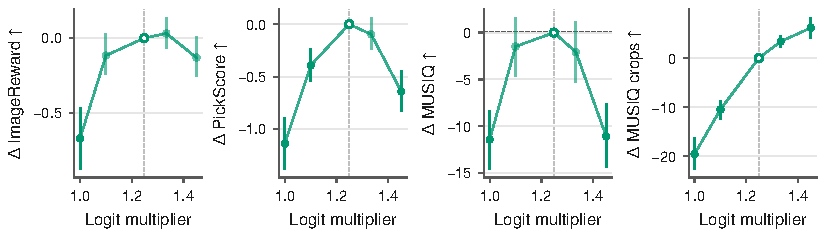
\includegraphics[width=\linewidth]{figs/strengthen/fs_sweep.pdf}
\caption{\textbf{Temperature sweep.} \tempsb{} at five logit multipliers fixed before generation, minus the reference $s^{0.16}$ (hollow mark, dashed vertical), on held-out rows 8 to 62 ($n=\N{st@s@n}$, seed 0). Whiskers are nominal 95\% paired intervals; pale marks cover zero. Reward models and full-frame MUSIQ fall on both sides of $s^{0.16}$, while crop MUSIQ keeps rising with the multiplier.}
\label{fig:fs-sweep}
\end{figure}
% Generated by paper/tables/strengthen_tables.py. Do not edit by hand.
\begin{table}[!htbp]
\centering
\caption{\textbf{Fresh prompts.} Means of \segaofficial{}, in the shaded column, and paired differences from it on 150 unseen Aesthetic-4K training captions ($n=150$, seed 0), with nominal 95\% intervals; $^{*}$ marks Holm-adjusted $p\le0.05$ over 50 tests (5 arms by 10 metrics). Bold marks the best entry for a metric when its interval separates it from \segaofficial. Key result: \dype{} is the only arm that beats \segaofficial{} under Holm on crop MUSIQ ($+2.32$) and CLIP-IQA ($+0.024$) while losing ImageReward ($-0.166$) and PickScore ($-0.38$); \tempsb{} ties ImageReward ($-0.011$) and loses crop CLIP-IQA and slope error under Holm.}
\label{tab:strengthen-fresh-arms}
\scriptsize
\setlength{\tabcolsep}{1.8pt}
% Generated by paper/tables/strengthen_tables.py. Do not edit by hand.
% Caption: \textbf{Fresh prompts.} Means of \segaofficial{}, in the shaded column, and paired differences from it on 150 unseen Aesthetic-4K training captions ($n=150$, seed 0), with nominal 95\% intervals; $^{*}$ marks Holm-adjusted $p\le0.05$ over 50 tests (5 arms by 10 metrics). Bold marks the best entry for a metric when its interval separates it from \segaofficial. Key result: \dype{} is the only arm that beats \segaofficial{} under Holm on crop MUSIQ ($+2.32$) and CLIP-IQA ($+0.024$) while losing ImageReward ($-0.166$) and PickScore ($-0.38$); \tempsb{} ties ImageReward ($-0.011$) and loses crop CLIP-IQA and slope error under Holm.
\begin{tabular}{@{}l>{\columncolor{papertint}}rrrrrr@{}}
\toprule
Metric & \hdr{\sega{}\\(released)} & \hdr{\sega{} base\\+\,temp.} & \hdr{\sega{}\\base} & \hdr{\ntk{}\\+\,temp.} & \hdr{\dype{}\\\phantom{x}} & \hdr{\ntk{}\\\phantom{x}} \\
\midrule
ImageReward$\uparrow$ & \refcell{0.667} & \dcellT{-0.011}{-0.055}{+0.035} & \dcellW{-0.875^{*}}{-1.022}{-0.723} & \dcellT{-0.042}{-0.093}{+0.008} & \dcellW{-0.166^{*}}{-0.250}{-0.084} & \dcellW{-0.923^{*}}{-1.077}{-0.768} \\
PickScore$\uparrow$ & \refcell{\mathbf{22.56}} & \dcellW{-0.07}{-0.13}{-0.01} & \dcellW{-1.05^{*}}{-1.22}{-0.89} & \dcellW{-0.12^{*}}{-0.18}{-0.05} & \dcellW{-0.38^{*}}{-0.51}{-0.26} & \dcellW{-1.05^{*}}{-1.22}{-0.89} \\
CLIP$\uparrow$ & \refcell{27.70} & \dcellT{-0.18}{-0.45}{+0.09} & \dcellW{-2.50^{*}}{-3.05}{-1.97} & \dcellT{-0.25}{-0.52}{+0.00} & \dcellT{-0.12}{-0.48}{+0.25} & \dcellW{-2.51^{*}}{-3.05}{-1.98} \\
MUSIQ$\uparrow$ & \refcell{44.99} & \dcellW{-1.56}{-2.72}{-0.43} & \dcellW{-10.28^{*}}{-12.15}{-8.33} & \dcellT{-0.76}{-1.99}{+0.49} & \dcellT{-0.65}{-1.99}{+0.74} & \dcellW{-10.48^{*}}{-12.46}{-8.53} \\
MUSIQ\textsubscript{crop}$\uparrow$ & \refcell{58.66} & \dcellT{-0.64}{-1.32}{+0.03} & \dcellW{-13.15^{*}}{-14.99}{-11.42} & \dcellT{-0.55}{-1.15}{+0.07} & \dcellB{\mathbf{+2.32}^{*}}{+1.41}{+3.25} & \dcellW{-13.00^{*}}{-14.75}{-11.29} \\
CLIP-IQA$\uparrow$ & \refcell{0.590} & \dcellT{-0.007}{-0.017}{+0.002} & \dcellW{-0.024}{-0.040}{-0.007} & \dcellW{-0.012}{-0.022}{-0.002} & \dcellB{\mathbf{+0.024}^{*}}{+0.011}{+0.036} & \dcellW{-0.021}{-0.038}{-0.003} \\
CLIP-IQA\textsubscript{crop}$\uparrow$ & \refcell{0.583} & \dcellW{-0.023^{*}}{-0.033}{-0.013} & \dcellW{-0.024}{-0.040}{-0.008} & \dcellW{-0.028^{*}}{-0.039}{-0.017} & \dcellT{+0.011}{-0.002}{+0.025} & \dcellW{-0.018}{-0.035}{-0.002} \\
Spec.\ err.$\downarrow$ & \refcell{1.133} & \dcellT{+0.005}{-0.035}{+0.038} & \dcellW{+0.469^{*}}{+0.344}{+0.608} & \dcellT{+0.014}{-0.028}{+0.050} & \dcellT{-0.042}{-0.101}{+0.011} & \dcellW{+0.434^{*}}{+0.294}{+0.582} \\
Slope err.$\downarrow$ & \refcell{0.220} & \dcellW{+0.016^{*}}{+0.006}{+0.026} & \dcellT{+0.013}{-0.016}{+0.042} & \dcellT{+0.012}{-0.003}{+0.026} & \dcellW{+0.016}{+0.000}{+0.031} & \dcellT{+0.008}{-0.020}{+0.038} \\
Tiling$\downarrow$ & \refcell{0.0644} & \dcellB{-0.0058}{-0.0094}{-0.0022} & \dcellT{-0.0107}{-0.0225}{+0.0004} & \dcellT{-0.0014}{-0.0057}{+0.0030} & \dcellT{+0.0090}{-0.0026}{+0.0214} & \dcellT{-0.0062}{-0.0175}{+0.0048} \\
\bottomrule
\end{tabular}

\end{table}

% Generated by paper/tables/strengthen_tables.py. Do not edit by hand.
\begin{table}[!htbp]
\centering
\caption{\textbf{Seed replication.} Held-out rows 8 to 194 ($n=187$ prompts): \segaofficial{} means over seeds 0 to 2 (shaded column) and paired differences of \tempsb{} minus \segaofficial. The first difference column averages seeds 0, 1 and 2 within each prompt before the paired bootstrap; $^{*}$ marks Holm-adjusted $p\le0.05$ over its 10 metrics and bold marks the better arm where its interval excludes zero. The other columns are sensitivity analyses without Holm marks. Key result: Averaged over seeds, \tempsb{} minus \segaofficial{} is $+0.021$ [$-0.004$, $+0.044$] on ImageReward and $-0.000$ [$-0.035$, $+0.037$] on PickScore, and $-2.00$ [$-2.74$, $-1.30$] on full-frame MUSIQ (Holm); every single seed gives the same MUSIQ verdict.}
\label{tab:strengthen-seeds}
\scriptsize
\setlength{\tabcolsep}{1.8pt}
% Generated by paper/tables/strengthen_tables.py. Do not edit by hand.
% Caption: \textbf{Seed replication.} Held-out rows 8 to 194 ($n=187$ prompts): \segaofficial{} means over seeds 0 to 2 (shaded column) and paired differences of \tempsb{} minus \segaofficial. The first difference column averages seeds 0, 1 and 2 within each prompt before the paired bootstrap; $^{*}$ marks Holm-adjusted $p\le0.05$ over its 10 metrics and bold marks the better arm where its interval excludes zero. The other columns are sensitivity analyses without Holm marks. Key result: averaged over seeds, \tempsb{} minus \segaofficial{} is $+0.021$ [$-0.004$, $+0.044$] on ImageReward and $-0.000$ [$-0.035$, $+0.037$] on PickScore, and $-2.00$ [$-2.74$, $-1.30$] on full-frame MUSIQ (Holm); every single seed gives the same MUSIQ verdict.
\begin{tabular}{@{}l>{\columncolor{papertint}}rrrrrr@{}}
\toprule
Metric & \hdr{\sega{} (rel.)\\seeds 0 to 2} & \hdr{Seeds\\0, 1, 2} & \hdr{Seeds\\1, 2} & \hdr{Seed\\0} & \hdr{Seed\\1} & \hdr{Seed\\2} \\
\midrule
ImageReward$\uparrow$ & \refcell{1.227} & \dcellT{+0.021}{-0.004}{+0.044} & \dcellT{+0.018}{-0.007}{+0.042} & \dcellT{+0.026}{-0.014}{+0.068} & \dcellT{+0.008}{-0.023}{+0.038} & \dcellT{+0.029}{-0.005}{+0.064} \\
PickScore$\uparrow$ & \refcell{23.10} & \dcellT{-0.00}{-0.04}{+0.04} & \dcellT{-0.01}{-0.06}{+0.03} & \dcellT{+0.03}{-0.03}{+0.09} & \dcellT{+0.01}{-0.05}{+0.07} & \dcellT{-0.04}{-0.10}{+0.02} \\
CLIP$\uparrow$ & \refcell{29.14} & \dcellT{-0.02}{-0.18}{+0.12} & \dcellT{-0.04}{-0.22}{+0.13} & \dcellT{+0.02}{-0.19}{+0.23} & \dcellT{-0.14}{-0.38}{+0.08} & \dcellT{+0.06}{-0.15}{+0.27} \\
MUSIQ$\uparrow$ & \refcell{\mathbf{45.34}} & \dcellW{-2.00^{*}}{-2.74}{-1.30} & \dcellW{-1.96}{-2.81}{-1.20} & \dcellW{-2.09}{-3.25}{-0.97} & \dcellW{-2.14}{-3.23}{-1.14} & \dcellW{-1.77}{-2.66}{-0.98} \\
MUSIQ\textsubscript{crop}$\uparrow$ & \refcell{58.40} & \dcellT{-0.19}{-0.69}{+0.30} & \dcellT{-0.23}{-0.79}{+0.35} & \dcellT{-0.11}{-0.71}{+0.48} & \dcellT{-0.22}{-0.89}{+0.46} & \dcellT{-0.23}{-0.86}{+0.46} \\
CLIP-IQA$\uparrow$ & \refcell{\mathbf{0.600}} & \dcellW{-0.007}{-0.013}{-0.000} & \dcellT{-0.005}{-0.012}{+0.002} & \dcellW{-0.009}{-0.018}{-0.001} & \dcellT{-0.007}{-0.015}{+0.001} & \dcellT{-0.004}{-0.012}{+0.004} \\
CLIP-IQA\textsubscript{crop}$\uparrow$ & \refcell{\mathbf{0.585}} & \dcellW{-0.014^{*}}{-0.021}{-0.007} & \dcellW{-0.013}{-0.020}{-0.005} & \dcellW{-0.017}{-0.025}{-0.008} & \dcellW{-0.014}{-0.023}{-0.005} & \dcellW{-0.012}{-0.020}{-0.003} \\
Spec.\ err.$\downarrow$ & \refcell{\mathbf{1.057}} & \dcellW{+0.045^{*}}{+0.029}{+0.061} & \dcellW{+0.050}{+0.033}{+0.068} & \dcellW{+0.034}{+0.015}{+0.052} & \dcellW{+0.054}{+0.035}{+0.074} & \dcellW{+0.046}{+0.026}{+0.066} \\
Slope err.$\downarrow$ & \refcell{\mathbf{0.199}} & \dcellW{+0.023^{*}}{+0.014}{+0.033} & \dcellW{+0.023}{+0.014}{+0.033} & \dcellW{+0.024}{+0.013}{+0.034} & \dcellW{+0.023}{+0.011}{+0.034} & \dcellW{+0.024}{+0.013}{+0.035} \\
Tiling$\downarrow$ & \refcell{0.0669} & \dcellB{\mathbf{-0.0060}^{*}}{-0.0085}{-0.0033} & \dcellB{-0.0056}{-0.0088}{-0.0024} & \dcellB{-0.0068}{-0.0106}{-0.0028} & \dcellT{-0.0033}{-0.0076}{+0.0011} & \dcellB{-0.0078}{-0.0123}{-0.0040} \\
\bottomrule
\end{tabular}

\end{table}

% Generated by paper/tables/strengthen_tables.py. Do not edit by hand.
\begin{table}[!htbp]
\centering
\caption{\textbf{Checkpoint by guidance.} Official \dype{} code on development rows 0 to 7 (seed 42, 28 steps, $4096^2$). Each entry is a ratio of whitened luminance power (radial power times $f^2$, Hann window) at one lattice bin with a period of 8 to 64 pixels: geometric mean over the 8 prompts with a 95\% bootstrap interval on the logs. The historical statistic picks the bin on the \fluxdev{} image and is biased upward; the shared bin is picked once per prompt from the mean log spectrum of all four cells. Descriptive development evidence, not a held-out test. Key result: \fluxdev{} carries more lattice power than \krea{} at both matched guidance values; raising guidance from 3.5 to 4.5 lowers it on \fluxdev{} while the \krea{} interval covers 1, so guidance modulates the lattice but does not create the checkpoint gap.}
\label{tab:strengthen-ckpt}
\scriptsize
\setlength{\tabcolsep}{1.8pt}
% Generated by paper/tables/strengthen_tables.py. Do not edit by hand.
% Caption: \textbf{Checkpoint by guidance.} Official \dype{} code on development rows 0 to 7 (seed 42, 28 steps, $4096^2$). Each entry is a ratio of whitened luminance power (radial power times $f^2$, Hann window) at one lattice bin with a period of 8 to 64 pixels: geometric mean over the 8 prompts with a 95\% bootstrap interval on the logs. The historical statistic picks the bin on the \fluxdev{} image and is biased upward; the shared bin is picked once per prompt from the mean log spectrum of all four cells. Descriptive development evidence, not a held-out test. Key result: \fluxdev{} carries more lattice power than \krea{} at both matched guidance values; raising guidance from 3.5 to 4.5 lowers it on \fluxdev{} while the \krea{} interval covers 1, so guidance modulates the lattice but does not create the checkpoint gap.
\begin{tabular}{@{}l rr@{}}
\toprule
Power ratio at the lattice bin & \hdr{Geometric\\mean} & \hdr{95\%\\interval} \\
\midrule
\multicolumn{3}{@{}l}{\emph{Historical F5 statistic, peak bin chosen on the \fluxdev{} image}} \\
\fluxdev/\krea, guidance $3.5$ & $12.0\times$ & $[7.8, 18.6]$ \\
\fluxdev/\krea, guidance $4.5$ & $7.4\times$ & $[4.5, 12.7]$ \\
\midrule
\multicolumn{3}{@{}l}{\emph{Shared bin, chosen on the mean of all four cells}} \\
\fluxdev/\krea, guidance $3.5$ & $11.6\times$ & $[7.5, 18.5]$ \\
\fluxdev/\krea, guidance $4.5$ & $6.7\times$ & $[4.2, 11.7]$ \\
Guidance $4.5/3.5$, \fluxdev & $0.52\times$ & $[0.41, 0.64]$ \\
Guidance $4.5/3.5$, \krea & $0.89\times$ & $[0.67, 1.11]$ \\
\bottomrule
\end{tabular}

\end{table}

% Generated by paper/tables/strengthen_tables.py. Do not edit by hand.
\begin{table}[!htbp]
\centering
\caption{\textbf{Default flow shift.} \segaofficial{} on development rows 0 to 7 (seed 0, 28 steps, guidance 4.5, $4096^2$) with the official shift ($\mu=1.15$, shaded) and with the diffusers default, which extrapolates $\mu$ to 11.55 at 65{,}536 image tokens. Means over 8 prompts, bold best; the last column is the paired difference with a nominal 95\% interval. Descriptive development evidence. Key result: the default shift worsens all ten metrics and lowers ImageReward by 3.70 [3.42, 3.96].}
\label{tab:strengthen-default-shift}
\scriptsize
\setlength{\tabcolsep}{1.8pt}
% Generated by paper/tables/strengthen_tables.py. Do not edit by hand.
% Caption: \textbf{Default flow shift.} \segaofficial{} on development rows 0 to 7 (seed 0, 28 steps, guidance 4.5, $4096^2$) with the official shift ($\mu=1.15$, shaded) and with the diffusers default, which extrapolates $\mu$ to 11.55 at 65{,}536 image tokens. Means over 8 prompts, bold best; the last column is the paired difference with a nominal 95\% interval. Descriptive development evidence. Key result: the default shift worsens all ten metrics and lowers ImageReward by 3.70 [3.42, 3.96].
\begin{tabular}{@{}l>{\columncolor{papertint}}rrr@{}}
\toprule
Metric & \hdr{Official\\$\mu=1.15$} & \hdr{Default\\$\mu=11.55$} & \hdr{Default\\$-$ official} \\
\midrule
ImageReward$\uparrow$ & \refcell{\mathbf{1.423}} & \refcell{-2.278} & \dcellW{-3.701}{-3.959}{-3.419} \\
PickScore$\uparrow$ & \refcell{\mathbf{23.41}} & \refcell{17.19} & \dcellW{-6.22}{-7.11}{-5.42} \\
CLIP$\uparrow$ & \refcell{\mathbf{30.32}} & \refcell{14.62} & \dcellW{-15.70}{-18.55}{-12.65} \\
MUSIQ$\uparrow$ & \refcell{\mathbf{42.49}} & \refcell{22.44} & \dcellW{-20.05}{-24.68}{-13.86} \\
MUSIQ\textsubscript{crop}$\uparrow$ & \refcell{\mathbf{58.23}} & \refcell{33.82} & \dcellW{-24.42}{-29.71}{-19.39} \\
CLIP-IQA$\uparrow$ & \refcell{\mathbf{0.557}} & \refcell{0.377} & \dcellW{-0.180}{-0.269}{-0.080} \\
CLIP-IQA\textsubscript{crop}$\uparrow$ & \refcell{\mathbf{0.580}} & \refcell{0.372} & \dcellW{-0.208}{-0.266}{-0.146} \\
Spec.\ err.$\downarrow$ & \refcell{\mathbf{0.857}} & \refcell{2.906} & \dcellW{+2.049}{+1.410}{+2.706} \\
Slope err.$\downarrow$ & \refcell{\mathbf{0.099}} & \refcell{0.499} & \dcellW{+0.400}{+0.256}{+0.542} \\
Tiling$\downarrow$ & \refcell{\mathbf{0.0894}} & \refcell{0.1329} & \dcellW{+0.0435}{+0.0259}{+0.0646} \\
\bottomrule
\end{tabular}

\end{table}



\FloatBarrier
\section{Seed-1 replication}\label{app:seed1}

This appendix reports the early seed-1 replication; \cref{tab:strengthen-seeds} in \cref{app:confirm} gives the later three-seed analysis of \cref{sec:confirm}. \Cref{tab:seed1} repeats the comparison for \tempsb{} and \constancytm{} on held-out rows 8--62 with a second seed, next to seed~0 on the same \N{so@n@tsb} prompts. One of the verdicts that changes, crop CLIP-IQA for \tempsb{} at seed 1, rests on an interval that excludes zero by less than $10^{-4}$, so the agreement count can move by one under another bootstrap seed. Every verdict that changes moves between a tie and a one-sided verdict. Spectral log-RMSE differences grow at seed 1 (\tempsb: \sod{tsb}{spec} against \hsd{tsb}{spec} at seed 0 on the same prompts; \constancytm: \sod{ctm}{spec} against \hsd{ctm}{spec}).

\begin{table}[!htbp]
\centering
\caption{\textbf{Seed 1 repeats most nominal seed-0 verdicts.} Paired differences against \segaofficial{} on the same \N{so@n@tsb} held-out prompts (rows 8--62) at seed 0 and at seed 1. \N{so@agree} of \N{so@cells} nominal verdicts agree. Intervals and direction triangles use the nominal 95\% convention of \cref{tab:main}; this descriptive table has no Holm adjustment.}
\label{tab:seed1}
\scriptsize
\setlength{\tabcolsep}{4pt}
\begin{tabular}{@{}l rr rr@{}}
\toprule
 & \multicolumn{2}{c}{\tempsb{} $-$ \segaofficial} & \multicolumn{2}{c}{\constancytm{} $-$ \segaofficial} \\
\cmidrule(lr){2-3}\cmidrule(lr){4-5}
Metric & seed 0 & seed 1 & seed 0 & seed 1 \\
\midrule
ImageReward$\uparrow$ & \dcellT{+0.070}{-0.011}{+0.160} & \dcellT{+0.031}{-0.036}{+0.094} & \dcellT{+0.063}{-0.014}{+0.142} & \dcellT{+0.019}{-0.045}{+0.083} \\
PickScore$\uparrow$ & \dcellT{+0.05}{-0.07}{+0.20} & \dcellT{+0.00}{-0.12}{+0.13} & \dcellT{-0.01}{-0.12}{+0.12} & \dcellT{-0.08}{-0.20}{+0.05} \\
CLIP$\uparrow$ & \dcellT{-0.02}{-0.54}{+0.47} & \dcellT{+0.02}{-0.40}{+0.46} & \dcellT{-0.31}{-0.82}{+0.17} & \dcellT{-0.32}{-0.78}{+0.13} \\
MUSIQ$\uparrow$ & \dcellW{-3.62}{-5.84}{-1.52} & \dcellW{-2.79}{-4.58}{-0.95} & \dcellW{-4.36}{-6.57}{-2.32} & \dcellW{-3.53}{-5.38}{-1.69} \\
MUSIQ\textsubscript{crop}$\uparrow$ & \dcellT{+0.43}{-0.53}{+1.40} & \dcellT{+0.35}{-0.69}{+1.44} & \dcellW{-1.77}{-2.82}{-0.77} & \dcellW{-1.99}{-3.09}{-0.91} \\
CLIP-IQA$\uparrow$ & \dcellT{+0.002}{-0.012}{+0.017} & \dcellT{-0.008}{-0.023}{+0.008} & \dcellW{-0.018}{-0.034}{-0.002} & \dcellW{-0.025}{-0.043}{-0.007} \\
CLIP-IQA\textsubscript{crop}$\uparrow$ & \dcellT{-0.008}{-0.024}{+0.009} & \dcellW{-0.015}{-0.032}{-0.000} & \dcellW{-0.034}{-0.050}{-0.015} & \dcellW{-0.042}{-0.059}{-0.025} \\
Spec.\ err.$\downarrow$ & \dcellW{+0.056}{+0.020}{+0.091} & \dcellW{+0.080}{+0.042}{+0.120} & \dcellW{+0.042}{+0.006}{+0.077} & \dcellW{+0.062}{+0.026}{+0.101} \\
Slope err.$\downarrow$ & \dcellW{+0.035}{+0.018}{+0.053} & \dcellW{+0.028}{+0.005}{+0.050} & \dcellW{+0.029}{+0.013}{+0.046} & \dcellW{+0.025}{+0.004}{+0.046} \\
Tiling$\downarrow$ & \dcellB{-0.0097}{-0.0157}{-0.0038} & \dcellT{-0.0055}{-0.0136}{+0.0027} & \dcellB{-0.0098}{-0.0156}{-0.0040} & \dcellT{-0.0058}{-0.0139}{+0.0023} \\
\bottomrule
\end{tabular}

\end{table}

\section{Partial and dev-only runs (not held-out results)}\label{app:partial}

This appendix expands \cref{sec:protocol,sec:papercode} with the runs behind the dev gate and the pilot. Nothing in it is a held-out result of the main protocol. The first subsection reports a held-out run that covers only part of the held-out set and started before the protocol was fixed; the other two report dev-prompt selection evidence and a descriptive pilot.

\subsection{Partial held-out run of \constancy}

The original \constancy{} was generated on \hon{cons} of the \N{ho@nprompts} held-out prompts (seed 0) before the protocol was fixed (\cref{app:dev}). Every number in this subsection comes from those \hon{cons} prompts only, and differences are paired on them. Against \segaofficial{} the run ties on the reward models, loses \hoa{cons}{musiq} full-frame MUSIQ points, gains crop MUSIQ (\hod{cons}{musiqc}) and has a much larger spectral error (\hod{cons}{spec}), with excess power in the top octaves and the largest excess of any arm in band 8 (log-power error \N{oct@cons@b8}; \cref{tab:octave}). Measured as a share of the gain of \segaofficial{} over \ntk{} on the same prompts ($n=\N{shx@n@cons}$), it recovers \N{shx@p@cons@musiqc}\%~\N{shx@ci@cons@musiqc} on crop MUSIQ but \N{shx@p@cons@musiq}\%~\N{shx@ci@cons@musiq} on full-frame MUSIQ.

The visibility gate of \cref{sec:laws} opens late on these prompts as on the dev prompts. On the \NmechConstN{} held-out prompts it opens only after the first $\NmechConstOnsetStepMed$ of $\NmechSteps$ steps (median; range $\NmechConstOnsetStepMin$ to $\NmechConstOnsetStepMax$), at $\sigma=\NmechConstOnsetSigmaMed$ (range $\NmechConstOnsetSigmaHi$ to $\NmechConstOnsetSigmaLo$), and the correction then acts in a median of $\NmechConstActiveStepsMed$ steps.

This partial run offers suggestive evidence about temperature. \ntk{} and \tempsb{} differ in both base and temperature, while \constancy{} adds to the \ntk{} base the log-$N$ temperature ($\tau=\N{c@taulogn}$) and a per-band correction that stays at zero for the first $\NmechConstOnsetStepMed$ of $\NmechSteps$ steps (median). On its \hon{cons} prompts it improves on \ntk{} by \hodci{consntk}{ir} ImageReward and \hodci{consntk}{musiqc} crop MUSIQ; on the same prompts, the entire \segaofficial{} minus \ntk{} gap is \hod{total41}{ir} ImageReward and \hod{total41}{musiqc} crop MUSIQ. The rows are a nonrandom manifest prefix, the temperature differs from \sega's, and the correction eventually acts. These observations alone do not separate base and temperature; the factorial of \cref{sec:decomp} does.

\subsection{Dev selection}\label{app:dev}

\Cref{tab:dev} lists every variant scored on the eight dev prompts, with its mean and its difference from the \segaofficial{} reference of the same campaign. These numbers chose what to run held-out; they are not results. Campaign 1 preceded the written gate: it sent \tempsb{} to the held-out set as a decomposition control and \constancytm{} as the candidate, and seven chunks of the original \constancy{} had already run on held-out rows when the protocol was fixed, which is why that arm has only \hon{cons} held-out prompts. Campaigns 2 and 3 applied the gate of \cref{sec:protocol}. In campaign 3 a fresh \segaofficial{} rerun served as the reference. It differs from the pilot run of the same prompts and seed by \N{dv@d@rerun@musiq} MUSIQ and \N{dv@d@rerun@ir} ImageReward, which is more than the MUSIQ margin by which the one passing variant cleared the gate (\N{dv@d@dev3segarmsnormalized@musiq}); we did not establish the source of the difference. That variant was not run on held-out prompts, and we make no claim about it. The dev set also misjudged the allocation itself: on the eight dev prompts \tempsb{} scored \N{dv@d@devsbtemponly@musiq} MUSIQ against \segaofficial, while held out it trails by \hoa{tsb}{musiq}.

\begin{table}[!htbp]
\centering
\caption{\textbf{Dev-set selection (rows 0--7, seed 0, $n=8$); selection evidence only.} Each cell: mean, and below it the difference from the campaign's \segaofficial{} reference. $^{a}$Partial held-out run (\hon{cons} prompts) started before the dev decision. $^{b}$Fresh rerun; the second line is its difference from the pilot run. $^{c}$Passed the dev gate; never evaluated on held-out prompts.}
\label{tab:dev}
\scriptsize
\setlength{\tabcolsep}{3pt}
\begin{tabular}{@{}l rrrrr l@{}}
\toprule
Variant & \makecell[r]{Image-\\Reward$\uparrow$} & \makecell[r]{MUSIQ\\full$\uparrow$} & \makecell[r]{CLIP\\score$\uparrow$} & \makecell[r]{Pick-\\Score$\uparrow$} & \makecell[r]{MUSIQ\\crop$\uparrow$} & Outcome \\
\midrule
\multicolumn{7}{@{}l}{\emph{Campaign 1 (reference: \segaofficial, pilot run)}} \\[1pt]
\segaofficial & \devcell{1.423}{+0.000} & \devcell{42.49}{+0.00} & \devcell{30.32}{+0.00} & \devcell{23.41}{+0.00} & \devcell{58.23}{+0.00} & reference \\
\tempntk & \devcell{1.282}{-0.141} & \devcell{40.36}{-2.13} & \devcell{29.96}{-0.36} & \devcell{23.12}{-0.29} & \devcell{60.29}{+2.05} & dev only \\
\constancy & \devcell{1.285}{-0.138} & \devcell{40.56}{-1.93} & \devcell{30.10}{-0.22} & \devcell{23.10}{-0.31} & \devcell{58.62}{+0.39} & partial held-out$^{a}$ \\
\constancytm{} on \ntk{} base, $\eta=1$ & \devcell{1.314}{-0.109} & \devcell{41.87}{-0.62} & \devcell{30.04}{-0.28} & \devcell{23.10}{-0.31} & \devcell{57.51}{-0.72} & dev only \\
\constancytm{} on \ntk{} base, $\eta=2$ & \devcell{1.313}{-0.110} & \devcell{43.34}{+0.85} & \devcell{30.13}{-0.19} & \devcell{23.04}{-0.37} & \devcell{54.61}{-3.63} & dev only \\
\tempsb & \devcell{1.444}{+0.021} & \devcell{42.72}{+0.24} & \devcell{30.32}{+0.00} & \devcell{23.26}{-0.15} & \devcell{55.93}{-2.30} & held-out (control) \\
\constancytm & \devcell{1.432}{+0.009} & \devcell{41.65}{-0.84} & \devcell{30.24}{-0.08} & \devcell{23.25}{-0.16} & \devcell{54.57}{-3.66} & held-out (candidate) \\
\addlinespace[2pt]
\multicolumn{7}{@{}l}{\emph{Campaign 2, written gate (reference: \segaofficial, pilot run)}} \\[1pt]
\aliastemp & \devcell{1.281}{-0.142} & \devcell{35.81}{-6.68} & \devcell{29.37}{-0.95} & \devcell{23.06}{-0.35} & \devcell{63.66}{+5.43} & fails gate \\
\aliastemps & \devcell{1.277}{-0.146} & \devcell{44.97}{+2.48} & \devcell{30.24}{-0.08} & \devcell{23.47}{+0.06} & \devcell{58.73}{+0.49} & fails gate \\
\segactm, $\eta=0.5$ & \devcell{1.441}{+0.018} & \devcell{42.48}{-0.01} & \devcell{30.20}{-0.12} & \devcell{23.31}{-0.10} & \devcell{58.51}{+0.27} & fails gate \\
\segactm, $\eta=1$ & \devcell{1.449}{+0.026} & \devcell{42.51}{+0.02} & \devcell{30.34}{+0.02} & \devcell{23.33}{-0.08} & \devcell{58.28}{+0.04} & passes, held-out \\
\addlinespace[2pt]
\multicolumn{7}{@{}l}{\emph{Campaign 3, same gate (reference: \segaofficial, fresh rerun)}} \\[1pt]
\segaofficial{} (rerun) & \devcell{1.391}{-0.032} & \devcell{43.28}{+0.79} & \devcell{30.15}{-0.17} & \devcell{23.38}{-0.03} & \devcell{58.59}{+0.36} & reference$^{b}$ \\
\segarms & \devcell{1.428}{+0.036} & \devcell{43.67}{+0.39} & \devcell{30.08}{-0.07} & \devcell{23.31}{-0.07} & \devcell{58.38}{-0.21} & passes, not confirmed$^{c}$ \\
\segauniform & \devcell{1.374}{-0.017} & \devcell{41.71}{-1.57} & \devcell{30.73}{+0.59} & \devcell{23.29}{-0.08} & \devcell{58.07}{-0.52} & fails gate \\
\segalag & \devcell{1.411}{+0.019} & \devcell{43.06}{-0.22} & \devcell{30.16}{+0.01} & \devcell{23.32}{-0.05} & \devcell{58.44}{-0.15} & fails gate \\
\bottomrule
\end{tabular}

\end{table}

\subsection{SEGA paper versus code: pilot numbers}\label{app:pilot}

In an eight-prompt pilot on the dev prompts, which is descriptive only, our implementation of the printed equations scores ImageReward \pim{segap}{ir}, CLIP \pim{segap}{clip} and full-frame MUSIQ \pim{segap}{musiq}, against \pim{sega}{ir}, \pim{sega}{clip} and \pim{sega}{musiq} for the released code (\cref{tab:pilot}). Freezing the printed allocation into a static tilt, a natural ablation of content adaptivity, destroys the images: CLIP falls to \pim{segapst}{clip} and logit gains reach $\NmechSegaStaticGainMax$. Freezing the released allocation instead costs much less (CLIP \pim{segast}{clip}, ImageReward \pim{segast}{ir}). \Cref{fig:papercode} in \cref{app:figs} shows the two gain trajectories and the resulting images. The pilot also ran \yarn{}, which follows a literal reading of a design note rather than the usual rotation-count convention.

\begin{table}[!htbp]
\centering
\caption{\textbf{Eight-prompt pilot on the dev prompts (rows 0--7, seed 0), descriptive only.} Means; triangles mark nominal paired bootstrap intervals against \segaofficial{} that exclude zero in the better or worse direction, which with $n=8$ is indicative at best. Static variants freeze the allocation instead of reading the current latent.}
\label{tab:pilot}
\scriptsize
\setlength{\tabcolsep}{2.4pt}
\begin{tabular}{@{}l rrrrrrr@{}}
\toprule
Method & \makecell[r]{Image-\\Reward$\uparrow$} & \makecell[r]{Pick-\\Score$\uparrow$} & \makecell[r]{CLIP\\score$\uparrow$} & \makecell[r]{MUSIQ\\full$\uparrow$} & \makecell[r]{MUSIQ\\crop$\uparrow$} & \makecell[r]{CLIP-IQA\\full$\uparrow$} & \makecell[r]{Spectral\\error$\downarrow$} \\
\midrule
\segaofficial & \refcell{1.423} & \refcell{23.41} & \refcell{30.32} & \refcell{42.49} & \refcell{58.23} & \refcell{0.557} & \refcell{0.857} \\
\segaofficialstatic & \mcellP{1.255}{w} & \mcellP{23.12}{t} & \mcellP{29.98}{t} & \mcellP{43.25}{t} & \mcellP{57.75}{t} & \mcellP{0.559}{t} & \mcellP{0.870}{t} \\
\segapaper & \mcellP{0.964}{w} & \mcellP{22.18}{w} & \mcellP{28.14}{w} & \mcellP{30.78}{w} & \mcellP{42.73}{w} & \mcellP{0.455}{w} & \mcellP{0.944}{t} \\
\segapaperstatic & \mcellP{-2.277}{w} & \mcellP{16.93}{w} & \mcellP{13.06}{w} & \mcellP{28.49}{w} & \mcellP{35.53}{w} & \mcellP{0.435}{w} & \mcellP{4.369}{w} \\
\addlinespace[2pt]
\ntk & \mcellP{0.757}{w} & \mcellP{22.37}{w} & \mcellP{27.84}{w} & \mcellP{32.91}{w} & \mcellP{41.41}{w} & \mcellP{0.543}{t} & \mcellP{1.220}{w} \\
\yarn & \mcellP{-0.163}{w} & \mcellP{21.14}{w} & \mcellP{28.06}{w} & \mcellP{42.51}{t} & \mcellP{66.69}{b} & \mcellP{0.645}{b} & \mcellP{1.250}{w} \\
\dype & \mcellP{1.118}{w} & \mcellP{22.23}{w} & \mcellP{28.59}{w} & \mcellP{44.38}{t} & \mcellP{58.32}{t} & \mcellP{0.584}{t} & \mcellP{0.920}{t} \\
\tempntk & \mcellP{1.282}{w} & \mcellP{23.12}{t} & \mcellP{29.96}{t} & \mcellP{40.36}{t} & \mcellP{60.29}{t} & \mcellP{0.578}{t} & \mcellP{1.038}{w} \\
\constancy & \mcellP{1.285}{w} & \mcellP{23.10}{t} & \mcellP{30.10}{t} & \mcellP{40.56}{t} & \mcellP{58.62}{t} & \mcellP{0.563}{t} & \mcellP{1.017}{w} \\
\bottomrule
\end{tabular}

\end{table}

\section{Implementation details}\label{app:impl}

This appendix expands \cref{sec:methods,sec:protocol}: \cref{tab:methods} expands \cref{tab:knobs}, the paragraphs below give the pipeline, the MUSIQ input, source versions and every arm's formula behind \cref{alg:sega,alg:ctm}, and \cref{app:laws} gives the per-band laws.

\begin{table}[!htbp]
\centering
\caption{\textbf{Arms, their knobs and sample sizes (expands \cref{tab:knobs}).} Temperature is the logit gain at $4096^2$; t/x: varies with the noise level / with the image. Held-out arms ran on rows 8--194, the pilot and dev arms only on the eight dev prompts. The shaded row is the reference, \segaofficial. Key result: \tempsb{} matches \segaofficial{} in base and temperature and drops only the per-band gain.}
\label{tab:methods}
\footnotesize
\setlength{\tabcolsep}{2.6pt}
\begin{tabular}{@{}l l c c c l@{}}
\toprule
Arm & Frequency base & Temperature & Per-band gain & t/x & $n$ \\
\midrule
\ntk & $\theta\,s^{2D/(D-2)}$ & none & none & no / no & \N{ho@nprompts} \\
\dype & PI/NTK ramps in $\sigma$ & $\N{c@dypegain}$ (spatial) & none & yes / no & \N{ho@nprompts} \\
\rowcolor{papertint}\segaofficial & $\theta\,s^{2D/(D-2)}/(1{+}0.1\ln s)$ & $s^{0.16}=\N{c@segatemp}$ & sensor, $\ge1$ & yes / yes & \N{ho@nprompts} \\
\segapaper & $\theta\,s^{2D/(D-2)}$ & $s^{0.16}$ & sensor, unbounded & yes / yes & 8 (pilot) \\
\tempsb & as \segaofficial & $s^{0.16}$ on all dims & none & no / no & \N{ho@nprompts} \\
\constancy & as \ntk & $\tau_N=\N{c@taulogn}$ & gated, late target & yes / yes & \hon{cons} (partial) \\
\constancytm & as \segaofficial & $s^{0.16}$ & gated, time-matched & yes / yes & \N{ho@nprompts} \\
\aliastemp & as \segaofficial & none & alias count, static & no / no & 8 (dev) \\
\segactm & as \segaofficial & $s^{0.16}$ & \sega{} $\times$ time-matched & yes / yes & \N{ho@nprompts} \\
\bottomrule
\end{tabular}
\end{table}

\begin{table}[!htbp]
\centering
\caption{\textbf{Configuration shared by every arm.} Gray bands group model, sampling and evaluation settings from the pipeline description below; \cref{tab:methods} lists what differs between arms. Key result: the arms differ only in rotary frequencies and gains.}
\label{tab:config}
\footnotesize
\setlength{\tabcolsep}{4pt}
\begin{tabular}{@{}l l@{}}
\toprule
\rowcolor{black!7}\multicolumn{2}{@{}l}{\textit{Model}} \\
Transformer & \krea{}, 19 double-stream and 38 single-stream blocks \\
Attention & 24 heads of dimension 128; rotary blocks of 16, 56 and 56 dimensions \\
Text encoders and autoencoder & T5 (512 tokens) and CLIP; \fluxdev{} autoencoder with tiled decoding \\
\rowcolor{black!7}\multicolumn{2}{@{}l}{\textit{Sampling}} \\
Resolution & $4096\times4096$, a $\N{c@tokside}^2$ token grid \\
Sampler & \N{c@steps} Euler flow-matching steps, flow shift $\mu=\N{c@muofficial}$, distilled guidance 4.5 \\
Precision and batch & bfloat16, batch size one, per-prompt CPU seed \\
\rowcolor{black!7}\multicolumn{2}{@{}l}{\textit{Evaluation}} \\
Prompts & \afk{} rows 0--7 (dev) and 8--194 (held-out, $n=\N{ho@nprompts}$) \\
Seeds & 0 for every arm; 1 on rows 8--62 for three arms \\
Statistics & paired percentile bootstrap, 2,000 resamples, generator seed 0 \\
Software & diffusers 0.39, PyTorch 2.11, pyiqa 0.1.16 \\
\bottomrule
\end{tabular}
\end{table}

\paragraph{Pipeline}
The \krea{} transformer, loaded through an environment override (\texttt{CROPE\_\allowbreak TRANSFORMER}), runs inside the \fluxdev{} pipeline (T5 and CLIP text encoders with 512 T5 tokens, autoencoder with tiled decoding at $4096^2$), diffusers 0.39~\citep{vonplaten2022diffusers}, PyTorch 2.11, bfloat16, batch size one, a per-prompt CPU seed, \N{c@steps} Euler steps and distilled guidance 4.5. The transformer has 19 double-stream and 38 single-stream blocks with 24 heads of dimension 128, and normalizes q and k before the rotation. Every arm multiplies q and k of every token in every block by one gain vector after the rotation; the vector is shared by blocks and heads and recomputed once per model call. The scheduler patch that holds $\mu=\N{c@muofficial}$ is applied before any configuration is recorded. The per-image JSON records hard-code the base model name and an attention label; the loaded transformer comes from the task scripts and the attention policy from the code revision (\cref{sec:pitfalls,app:compute}).

\paragraph{MUSIQ input pipeline}
We use pyiqa 0.1.16's KonIQ10k MUSIQ model. The project passes RGB float32 values in $[0,1]$ without resizing; MUSIQ normalizes to $[-1,1]$ and combines the native image with aspect-preserving 224- and 384-pixel views, resized by bicubic interpolation with \texttt{align\_corners=False} and \texttt{antialias=False}. Each scale is split into $32\times32$ patches at stride 32, with SAME padding where needed. The native setting \texttt{max\_seq\_len\_from\_original\_res=-1} retains all patches: a $4096^2$ frame contributes 16,384 native patches, plus 49 and 144 resized-view patches, for 16,577 before the class token. A $1024^2$ crop contributes 1,217. Neither native square grid needs padding. The spatial embedding's $10\times10$ hash grid does not downsample the image. We verified these counts by executing the installed preprocessor without loading model weights. Crop MUSIQ averages four separately scored, fixed random $1024^2$ crops shared across methods. Full-frame MUSIQ is thus a multiscale quality score that includes every native pixel, not a direct sharpness measurement.

\paragraph{Source versions}
Our \sega{} comparison uses \href{https://github.com/rajabi2001/sega/tree/ddaab08552c7b7ceba2ebd8f579a0f65dee90b5e}{released commit \texttt{ddaab08552c7}}. The allocation is in \texttt{flux\_sega/transformer\_flux.py}, lines 103--154; projected-feature sensing follows the input projection in the same file. Our printed-law implementation follows Section 4.1 and equations (3)--(7) of \citet{sega2026}, with the strengthened base from equation (9) in its Appendix A.2.2. The six-row comparison in \cref{tab:papercode} (\cref{sec:papercode}) records our interpretation, including how the unspecified index axis and latent input are implemented. We did not obtain confirmation of that interpretation from the authors. Our \dype{} port and official-code diagnostic use \href{https://github.com/guyyariv/DyPE/tree/436fe612fb7695fa2d5dc32d63390c048ba6033c}{commit \texttt{436fe612fb76}}.


\paragraph{Printed \sega{} equations}
\sega~\citep{sega2026} reads the spectrum of its input at every model call and sets per-pair gains around a reference gain $m_{\mathrm{ref}}=s^{0.08}$. In the printed equations, the energy $E_a$ of the channel-mean latent at pair $j$'s frequency bin is standardized across pairs, $z_{a,j}$, and
\begin{equation}
\begin{aligned}
m_{a,j}&=m_{\mathrm{ref}}\bigl(1-\varsigma\,u_{a,j}\bigr),
&\varsigma&=1-\mathrm{SF}(E_{\mathrm{iso}})^{1.5},\\
u_{a,j}&=\tanh z_{a,j}-\operatorname{mean}_i\tanh z_{a,i},
\end{aligned}
\label{eq:sega}
\end{equation}
where $\mathrm{SF}$ is the flatness of the radial spectrum. Low-energy pairs, usually the fast ones, thus gain attention weight in proportion to how far the spectrum is from flat. Our reading of the printed formulation differs from the release at each of the six stages in \cref{tab:papercode}. We call its parity-tested port \segaofficial{} and our implementation of the printed equations \segapaper; static variants use the mean allocation over pilot prompts and steps.

\paragraph{\dype}
For spatial axis $a$ with scale $s$ and $\kappa=\sigma^2$, let $b(r)=D\ln\bigl(64/(2\pi r)\bigr)/(2\ln\theta)$ be the pair index that completes $r$ rotations over 64 tokens and $\mu_{r_1,r_2}(j)=1-\operatorname{clip}\bigl((j-\ell)/(h-\ell),0,1\bigr)$ with $\ell=\max(\lfloor b(r_1)\rfloor,0)$ and $h=\min(\lceil b(r_2)\rceil,D/2)$. Then
\[
\begin{aligned}
\omega^{\mathrm{mix}}_j&=\tfrac{\omega_j}{s}\bigl(1-\mu_{1.25\kappa,0.75\kappa}(j)\bigr)+\omega^{\mathrm{ntk}}_j\,\mu_{1.25\kappa,0.75\kappa}(j),\\
\omega'_j&=\omega^{\mathrm{mix}}_j\bigl(1-\mu_{16\kappa,2\kappa}(j)\bigr)+\omega_j\,\mu_{16\kappa,2\kappa}(j),
\end{aligned}
\]
where $\omega^{\mathrm{ntk}}$ are the NTK-aware frequencies; the spatial cos/sin amplitude is $1+0.1\ln s$, as in the official code at the inspected revision.

\paragraph{\segaofficial}
The sensor takes the channel mean $Z$ of the projected input features on the token grid. The axis profile $E_a$ is the one-dimensional FFT power along axis $a$ averaged over the other axis and rebinned into $K_a=\max(\lfloor L_a/2\rfloor,8)$ bins. Pair $j$ reads $\ell_j=\ln E_a\bigl((1-\rho_j)(K_a-1)\bigr)$ by linear interpolation, with $\rho_j=j/(D/2-1)$ the normalized rank of its log period; $z_j$ standardizes $\ell_j$ with the sample standard deviation; and $m_{a,j}=\max\bigl(1,m_{\mathrm{ref}}[1-0.15\,\varsigma\,c_j]\bigr)$ with $c_j=\tanh(1.5z_j)-\operatorname{mean}_i\tanh(1.5z_i)$, $m_{\mathrm{ref}}=\max(s,1)^{0.08}$ and $\varsigma=1-\mathrm{SF}^{1.5}$ from the radially binned two-dimensional power. The index axis keeps gain 1.

\begin{figure}[!htbp]
\centering
\figorplaceholder[\linewidth]{figs/fA_method_zoom.pdf}{3.5in}
\caption{\textbf{Both gain controllers at component level.} (a)~The released \sega{} sensor of \cref{fig:method}b reads the channel mean of the projected input features, maps the axis profile to rotary pairs by rank and scales its tilt by the radial flatness. (b)~\constancytm{} gates a bounded log-power correction toward the time-matched native target and adds it to the \sega{} temperature. White boxes are inputs and outputs; the equations repeat \cref{alg:sega,alg:ctm} and \cref{app:impl}.}
\label{fig:method_zoom}
\end{figure}

\subsection{Per-band control laws}\label{app:laws}

Each law sets $\ln g_{a,j}=\ln\tau+\Delta_{a,j}$, a temperature plus a bounded per-band correction. The diffusion noise level supplies the bandwise noise floor.

\paragraph{\constancy}
For half-octave bands $b$, a gate compares the current input's band energy with the known noise floor, $\rho_{a,b}=\max\bigl(E^{x}_{a}[b]/(\sigma^2C)-1,0\bigr)$ and $w_{a,b}=\rho_{a,b}/(1+\rho_{a,b})$, and an error compares the previous clean estimate's band energy $\hat E_a[b]$ with a native-resolution target $P^{\mathrm{nat}}$, the mean log spectrum of the model's own $1024^2$ samples on 16 calibration prompts outside the evaluation set:
\begin{equation}
e_{a,b}=\tfrac12\bigl(P^{\mathrm{nat}}_{a}(f_b)+c_a-\ln \hat E_{a}[b]\bigr),\qquad \delta_{a,b}=\eta\,w_{a,b}\operatorname{clip}(e_{a,b},-1,1),
\label{eq:constancy}
\end{equation}
where $c_a$ anchors the target level on visible bands of 16 to 64 token wavelengths. The pair correction $\Delta_{a,j}$ interpolates $\delta$ in $\log f$, with $\tau=\tau_N$ and $\eta=1$. A natural spectrum gives $e=0$ and reduces the law to the global temperature. The target is the native spectrum of the final, nearly clean steps.

\paragraph{\constancytm}
The same law with a time-matched target: $P^{\mathrm{nat}}(f,\sigma)$ is the clean estimate's native spectrum at the same noise level, tabulated over all \N{c@steps} native steps, so the anchor no longer needs the gate. Built on the base and temperature of \segaofficial, it isolates the allocation, with \tempsb{} as its control.

\paragraph{\aliastemp{} and \segactm}
\aliastemp{} applies the log-$N$ temperature pair by pair, taking as a pair's key pool the number of keys it can resolve on the grid (\cref{app:impl}); \aliastemps{} shifts all its log gains by one constant to match \sega's reference gain in geometric mean. \segactm{} multiplies the allocation of \segaofficial{} by the time-matched correction, $\ln g=\ln g^{\textsc{sega}}+\Delta$, with $\eta\in\{0.5,1\}$ on the dev set and $\eta=1$ held out.

\paragraph{Band energies and calibration}
Band energies are densities: with an orthonormal FFT, $P(k)=\sum_c|\mathcal F(x_c-\bar x_c)(k)|^2$, $E_a(k)$ averages $P$ over the other axis, and $E_a[b]$ averages over half-octave bands $b$ (13 bands at 256 tokens per side). Unit white noise gives $E_a[b]=C=64$ in expectation, so the noise floor at level $\sigma$ is $\sigma^2C$. The gate uses the current input; the error uses the clean estimate of the previous call, $\hat x_0=x_{n-1}-\sigma_{n-1}v_\theta(x_{n-1})$. Corrections are interpolated in $\log f$ between band centers and applied to pairs with frequency above one cycle per grid, which at $4096^2$ are pairs 0 to 8 of each axis. Step 0 has no clean estimate and uses the temperature alone, and $|\ln g-\ln\tau|\le\eta$ always. The native targets come from $1024^2$ samples of the same model on 16 Pick-a-Pic prompts~\citep{kirstain2023pickapic} disjoint from the evaluation set: the late target averages the three steps with $\sigma<0.3$, and the time-matched target keeps all 28 steps and is interpolated in $\sigma$.

\paragraph{\aliastemp}
\aliastemp{} applies the log-$N$ temperature of \cref{sec:background} pair by pair. A pair of wavelength $\lambda_{a,j}$ tokens under the released base, on a grid of $L$ tokens per side ($L=64$ at native size), gets the logit gain
\[
g_{a,j}=\frac{\ln\bigl(n(\lambda_{a,j},L)\,L\bigr)}{\ln\bigl(n(\lambda_{a,j},64)\cdot 64\bigr)},\qquad n(\lambda,L)=\min\bigl(L,\max(1,L/\lambda)\bigr),
\]
where $n(\lambda,L)$, the pair's alias count, is the number of its wavelengths across the grid, bounded by 1 and $L$; the index axis takes $\tau_N$. The gains are static and content-free, with no correction and no further temperature. \aliastemps{} shifts every $\ln g$ by one constant so that the mean over all 128 dimensions equals \sega's reference log gain, $0.16\ln s$.


\section{Mechanism diagnostics}\label{app:mech}

This appendix expands the diagnostic paragraph of \cref{sec:laws} with the figure, numbers and protocols behind it.

\begin{figure}[!htbp]
\centering
\figorplaceholder[\linewidth]{figs/f7_mechanism.pdf}{2.3in}
\caption{\textbf{Dev-prompt mechanism diagnostics.} The late-profile correction starts late, and the response to a band-gain change differs across prompts. (a)~Mean $|\ln g-\ln\tau|$ over spatial rotary pairs per step: median and interquartile band over eight dev prompts, seed 0, with both targets on the \ntk{} base. In the gray region the late-profile correction is exactly zero in all eight prompts (steps 1 to 19, $\sigma\geq 0.64$). \emph{Right:} median corrections for pairs 0--11; pairs 12--27 are identically zero. (b)~Width-axis response matrices for dev prompts 0 to 2, seed 0. Each cell is the same-seed finite-difference change in final-latent log power divided by $\ln(\NmechProbeFactor)$ when one input octave receives a $\NmechProbeFactor\times$ logit gain on both spatial axes throughout sampling. The matrices share one zero-centerd color scale and are not averaged across prompts; no seed-to-seed uncertainty is estimated.}
\label{fig:mechanism}
\end{figure}

The following gate and transfer-probe measurements use development prompts; the time-matched and released-allocation summaries use logged held-out trajectories. These diagnostics do not identify causal mediators of image quality.

\paragraph{The visibility gate opens too late}
\constancy's correction is exactly zero until a band with a wavelength of 16 to 64 tokens holds more than twice the noise power ($w>\tfrac12$). On the eight dev prompts it first becomes nonzero at $\sigma=\NmechConstDevOnsetSigmaHi$ and is nonzero on all of them only by $\sigma=\NmechConstDevOnsetSigmaLo$ (\cref{fig:mechanism}a). For most of sampling, including the steps that fix the layout, \constancy{} is thus the \ntk{} base with a log-$N$ temperature: the gate is principled, but at $4096^2$ the bands it guards stay below the noise floor until late.

\paragraph{A native-resolution target improves spectral match while lowering MUSIQ}
The time-matched target opens the gate early. On the held-out \constancytm{} runs, corrections exceed $\NmechMaterialThreshold$ in log gain after the first $\NmechTmMaterialStepMed$ steps (median), and $\NmechTmNegPct\%$ of all nonzero corrections are negative: they lower the mid pairs 6 to 8 ($\NmechTmCoarseFinal$ at the last step) and, late, the finest pairs 0 to 2 ($\NmechTmFineFinal$). These corrections reduce the gains of the corresponding rotary bands. Against \tempsb, output spectral errors shrink slightly while both MUSIQ scores fall. Matching a native spectrum and maximizing a learned quality score are different objectives; the measurements do not show which individual gain changes cause the score losses.

\paragraph{\sega's allocation is mostly a fixed tilt}
Across the held-out prompts the released logit gain stays between $\NmechSegaGainMin$ and $\NmechSegaGainMax$. A fixed tilt over pairs explains $\NmechSegaStaticPct\%$ of its variance and a tilt plus a per-step profile $\NmechSegaStaticTimePct\%$. The prompt-dependent remainder, $\NmechSegaContentPct\%$ overall and $\NmechSegaLateContentPct\%$ from step $\NmechLateFirstStep$ on, is an upper bound on content dependence, because it also contains each prompt's noise draw. At the last step the finest pair has a logit gain of $\NmechSegaFinalFineGain$ and the $\NmechSegaFinalClampPairs$ slowest pairs per axis sit at the clamp of 1. A law that adapts more to content therefore has little to copy: \segactm{} raises the prompt-dependent share to $\NmechCtmContentPct\%$ and gains nothing held out. A CPU study of the printed equations finds the same structure on another latent space (\cref{app:mech}).

\paragraph{The response to gain changes is weak and prompt-dependent}
Every law assumes that raising a band's gain raises its output power. A probe on three dev prompts that scales one octave's gain by $\NmechProbeFactor$ (\cref{fig:mechanism}b) finds a clear same-octave width-axis response for one prompt and a near-zero one for the other two, off-diagonal responses spread across octaves, and a weak height-axis response. On two dev prompts, a local linear model predicts half-step band-power changes little better than no change (\cref{app:mech}). These probes question a simple band-local response model, but their small sample does not establish a universal limit on per-band control.

\paragraph{CPU study of the printed \sega{} law}
Before running any model we measured the printed allocation (\cref{eq:sega}) on forward-noised latents of the FLUX.2 autoencoder for \NmechCpuN{} DIV2K crops. A fixed tilt over pairs explained $\NmechCpuStaticPct\%$ of the variance of the modulation, tilt plus timestep $\NmechCpuStaticTimePct\%$, leaving at most $\NmechCpuContentPct\%$ for content; the flatness gate $\varsigma$ was explained to $R^2=\NmechCpuSigmaTimeRsq$ by the timestep alone and to $\NmechCpuSigmaGenericRsq$ by a generic $1/f$ field. On our held-out \krea{} runs the released gate $\varsigma$ is likewise explained to $R^2=\NmechSegaSpreadTimeRsq$ by the timestep. The channel mean that the printed sensor reads keeps $\NmechCpuChanMeanPct\%$ of the latent power. In a blur sweep at $\sigma=\NmechBlurLowSigma$ over \NmechBlurN{} test crops, the printed law's contrast between fine and coarse pairs changed by $\NmechBlurSegaChangePct\%$ between no blur and a blur of \NmechBlurMax{} tokens, while an oracle version of the constancy law changed \NmechBlurConstFold-fold. These measurements motivated the constancy design; they use the printed law, another autoencoder and forward-noised rather than sampled latents, so we use them only as context for \cref{sec:laws}.

\paragraph{Probe protocol}
The transfer probe of \cref{fig:mechanism} reruns a dev prompt with the gain of one input octave multiplied by \NmechProbeFactor{} on both spatial axes, with the same seed, and reports the finite-difference elasticity $\partial\log P_{\mathrm{out}}/\partial\log g_{\mathrm{in}}$ for six input and seven output octaves of the final latent and image. It used the \ntk{} base with the log-$N$ temperature, three dev prompts and one seed. The local-response experiment applied half-step perturbations at steps 6, 14 and 22 of two dev prompts and compared the observed change in band power with the prediction of a locally fitted linear response: the median error relative to predicting no change was $\NmechCrSeventeenErrMed$ (range $\NmechCrSeventeenErrMin$ to $\NmechCrSeventeenErrMax$; \NmechCrSeventeenBelowOne{} of \NmechCrSeventeenAxisRows{} cases below 1). It tested a single octave, below the resolution of the token grid, so it does not cover all rotary bands. On the width axis of \krea, the mean diagonal elasticity of the transfer probe is $\NmechProbeLatWDiagA$ for one prompt but $\NmechProbeLatWDiagB$ and $\NmechProbeLatWDiagC$ for the other two, against a mean off-diagonal response of $\NmechProbeLatWOffAvg$.

\paragraph{Confounded cross-checkpoint probe}
Raising the fastest octave's gain gave a width-axis elasticity of $\NmechProbeLatWTopA$ on \krea{} and $\NmechFdevLatWTop$ on \fluxdev{} for one dev prompt. Guidance and code revision also differed, so we draw no conclusion about checkpoint-dependent response from the sign change.

\paragraph{Allocation controls on the dev set}
A third dev campaign replaced the allocation of \segaofficial{} by a uniform gain with the same root-mean-square value, or kept its shape and removed the rise in mean gain caused by the clamp. On the eight dev prompts the uniform control changed MUSIQ by $\NmechCrFourteenUniformMusiq$ and the shape-only control by $+\NmechCrFourteenNormMusiq$, while a rerun of \segaofficial{} itself moved MUSIQ by $+\NmechCrFourteenRepeatMusiq$. These differences are within run-to-run variation and were not taken to held-out prompts.

\paragraph{Diagnostics not reported}
The project also measured run-to-run repeatability of the gain histories, the sensitivity of \sega's sensor to channel-mean shifts at artificial states, attention-operator approximations and native-resolution semantic consistency. None bears on the claims of this paper, and we do not report them.

\section{Compute and timing}\label{app:compute}

This appendix expands the compute paragraph of \cref{sec:protocol}: \cref{tab:cost} summarizes the kernel and GPU effects, and \cref{tab:compute} gives the cost of every retained image.

\begin{table}[!htbp]
\centering
\caption{\textbf{Kernel and GPU set cost.} Median seconds per $4096^2$ sample; the FlashAttention-2 timings come from the dev pilot. \Cref{tab:compute} expands this table. Key result: the kernel changes cost far more than the method does.}
\label{tab:cost}
\scriptsize
\setlength{\tabcolsep}{3pt}
\begin{tabular}{@{}l r r@{}}
\toprule
Setting & s/image$\downarrow$ & relative \\
\midrule
\rowcolor{papertint}GH200, cuDNN SDPA & \NcompGHcudnnSec & 1.00 \\
GH200, FlashAttention-2 & \NcompGHflashSec & \NcompFlashRatio \\
GB200, same code & \NcompBWSec & $1/\NcompBWSpeedup$ \\
\bottomrule
\end{tabular}
\end{table}

On the same GH200 node and method, forcing FlashAttention-2 makes a $4096^2$ sample take \NcompFlashRatio{} times as long as cuDNN-first SDPA (medians \NcompGHflashSec\,s and \NcompGHcudnnSec\,s), while method families on one node differ by at most \NcompFamilySpreadPct\%; one GB200 GPU is \NcompBWSpeedup{} times faster than a GH200 (\cref{tab:compute}). The forced-FlashAttention-2 comparison uses development-pilot runs and is descriptive. Timings of different methods are comparable only with the kernel and the GPU fixed.

\Cref{tab:compute} gives the sampling cost of the \NcompNimgs{} retained $4096^2$ images, \NcompGPUhours{} GPU-hours in total (\NcompGPUhoursGH{} on GH200, \NcompGPUhoursBW{} on GB200), with a median peak allocation of \NcompPeakGB\,GB. The second campaign's dev runs and the held-out \segactm{} run used one GB200 node; every other run used GH200 nodes, and every forced-FlashAttention-2 timing at $4096^2$ comes from the eight-prompt pilot. The GPU of each image was recovered from task and fleet logs, and its attention policy from the code revision pinned by its implementation hash, because the records carry a constant attention label. % Generated by paper/tables/compute_table.py. Do not edit by hand.
The SDPA column of \cref{tab:compute} gives the requested backend policy (cuDNN first: cuDNN, then FlashAttention, then memory-efficient); the dispatched kernel was not logged. The \sega{} family comprises released and paper-equation \sega{} with their static ablations; the \segactm{} family, \segactm{} and its dev-only allocation controls; the \constancy{} family, \constancy{} and its dev sweeps, \constancytm{}, the temperature-only ablations, \aliastemp{} and \aliastemps{}. Node c619-102 ran 14\% slower than the other GH200 nodes under both kernels (median power 665\,W versus 836\,W while generating), so it is listed separately; the forced-FA2 \yarn{} and \dype{} pilots ran only there. The native rows run \krea{} without RoPE changes; the first image of each worker process carries a one-off warm-up (4.1\,s with cuDNN first, 0.9\,s with FA2), which widens the cuDNN-first IQR at $1024^2$. The official \dype{} script uses the default SDPA dispatch of diffusers.
 Timings exclude model loading (\NcompModelLoadSec\,s per worker process) and PNG writing, except the single official \dype{} run.

% Generated by paper/tables/compute_table.py. Do not edit by hand.
\begin{table}[t]
\centering
\small
\caption{\textbf{Sampling cost is set by the attention kernel and the GPU, not by the method.} On the same GH200 node and method, forced FlashAttention-2 (FA2) takes 1.54 times as long as cuDNN-first SDPA (290\,s versus 188\,s per $4096^2$ image), and one GB200 GPU is 2.01 times faster than a GH200 under cuDNN-first SDPA (93\,s). Method families on one node differ by at most 0.6\%. Node c619-102 ran 14\% slower than the other GH200 nodes under both kernels (median power 665\,W versus 836\,W while generating), so it is listed separately; the forced-FA2 \yarn{} and \dype{} pilots ran only there. $n$ counts images. Seconds cover prompt encoding, 28 denoising steps and VAE decoding, without model loading or PNG writing; IQR is the interquartile range; peak is \texttt{torch.cuda.max\_memory\_allocated}; GPU-h sums the per-image seconds. The SDPA column gives the requested backend policy (cuDNN first: cuDNN, then FlashAttention, then memory-efficient); the dispatched kernel was not logged. \sega{} family: released and paper-equation \sega{} with their static ablations. \segactm{} family: \segactm{} and its dev-only allocation controls. \constancy{} family: \constancy{} and its dev sweeps, \constancytm{}, the temperature-only ablations, \aliastemp{} and \aliastemps{}. The native rows run \krea{} without RoPE changes; the first image of each worker process carries a one-off warm-up (4.1\,s with cuDNN first, 0.9\,s with FA2), which widens the cuDNN-first IQR at $1024^2$. The official \dype{} script uses the default SDPA dispatch of diffusers, and its single timing also includes writing the PNG.}
\label{tab:compute}
\begin{tabular}{@{}llrrrrrr@{}}
\toprule
SDPA & Methods & $n$ & Nodes & Median (s) & IQR (s) & Peak (GB) & GPU-h \\
\midrule
\multicolumn{8}{@{}l}{\emph{$4096^2$, GH200 (10 nodes)}} \\
FA2, forced & \ntk & 8 & 1 & 289.8 & 289.8--289.9 & 40.8 & 0.6 \\
FA2, forced & \sega{} family & 23 & 3 & 289.8 & 289.7--290.1 & 40.8 & 1.9 \\
FA2, forced & \constancy{} family & 16 & 2 & 290.4 & 289.9--290.5 & 40.8 & 1.3 \\
cuDNN first & \ntk & 160 & 6 & 187.2 & 186.2--187.5 & 40.8 & 8.3 \\
cuDNN first & \dype & 167 & 6 & 187.9 & 187.6--188.1 & 40.8 & 8.7 \\
cuDNN first & \sega{} family & 197 & 9 & 187.8 & 187.5--188.2 & 40.8 & 10.3 \\
cuDNN first & \segactm{} family & 24 & 2 & 189.4 & 184.9--189.6 & 40.8 & 1.3 \\
cuDNN first & \constancy{} family & 532 & 8 & 187.9 & 187.6--188.6 & 40.8 & 27.8 \\
\addlinespace[3pt]
\multicolumn{8}{@{}l}{\emph{$4096^2$, GH200 node c619-102 (listed separately)}} \\
FA2, forced & \yarn, \dype & 16 & 1 & 329.6 & 329.5--329.7 & 40.8 & 1.5 \\
cuDNN first & all methods & 195 & 1 & 214.6 & 214.0--215.3 & 40.8 & 11.6 \\
\addlinespace[3pt]
\multicolumn{8}{@{}l}{\emph{$4096^2$, GB200 (1 node, 4 GPUs)}} \\
cuDNN first & \segactm{} family & 204 & 1 & 93.3 & 92.5--94.3 & 40.8 & 5.3 \\
cuDNN first & \constancy{} family & 16 & 1 & 93.2 & 92.1--93.3 & 40.8 & 0.4 \\
\addlinespace[3pt]
\multicolumn{8}{@{}l}{\emph{native $1024^2$, GH200, \krea{}}} \\
FA2, forced & no RoPE change & 16 & 1 & 5.47 & 5.47--5.48 &  & \\
cuDNN first & no RoPE change & 8 & 2 & 4.94 & 4.93--5.93 & 36.3 & \\
\addlinespace[3pt]
\multicolumn{8}{@{}l}{\emph{$4096^2$, GH200, official \dype{} script}} \\
default & \dype{} (official code) & 1 & 1 & 193.3 & & & \\
\bottomrule
\end{tabular}
\end{table}




\FloatBarrier
\section{Reproducibility checklist}\label{app:repro}

This appendix expands the reproducibility statement of the main text.
\begin{itemize}
\item \textbf{Numbers.} \texttt{paper/tables/strengthen\_tables.py} writes every confirmation number from the registered analysis outputs, which an independent recomputation from the raw evaluator scores matches within $10^{-14}$. \texttt{paper/tables/make\_tables.py} recomputes every held-out paired difference from the archived per-prompt scores, checks it against the registered analysis output (largest absolute difference below $10^{-15}$), and writes every table and every number cited in the text. \texttt{compute\_table.py} and \texttt{mechanism\_numbers.py} do the same for timings and mechanism statistics. Scratch inputs are snapshotted next to the scripts.
\item \textbf{Protocol.} Dev rows 0--7 and held-out rows 8--194 of the \afk{} evaluation captions; seed 0; seed-1 replication on rows 8--62; selection gate and its outcomes in \cref{app:dev}. The confirmation campaign follows a dated preregistration with amendments (factorial, sweep, \N{st@e@n} fresh training-split captions, seeds 1 and 2), whose complete tables are in \cref{app:confirm}.
\item \textbf{Generation.} Every image has a JSON sidecar with the full configuration, code revision, implementation hash, executed noise levels, per-step gains, wall time and peak memory.
\item \textbf{Statistics.} Paired percentile bootstrap, 2,000 resamples, generator seed 0, with nominal per-metric intervals. Stars in \cref{tab:main,tab:deltas_full} mark approximate centered-bootstrap tests adjusted by Holm within each table, and stars in the confirmation tables use the registered families of 3, 80, 40, 50 and 10 tests; the other descriptive tables retain nominal intervals.
\item \textbf{Third-party code.} \sega{} and \dype{} are re-implemented from their released code at pinned revisions with numerical parity tests; \dype{}'s official code was also run end to end for the checkpoint diagnosis.
\item \textbf{Not done.} No human study; one model family, since the registered \qwen{} test ran out of GPU memory; one resolution; one seed for most arms; FID and KID too noisy at these sample sizes to rank methods.
\end{itemize}
